\documentclass[a4paper]{report}

%====================== PACKAGES ======================

% Couleur tableaux
\usepackage[table]{xcolor}% http://ctan.org/pkg/xcolor

\usepackage[french]{babel}
\usepackage[utf8x]{inputenc}
%pour gérer les positionnement d'images
\usepackage{float}
\usepackage{amsmath}
\usepackage{graphicx}
\usepackage{url}
%pour les informations sur un document compilé en PDF et les liens externes / internes
\usepackage{hyperref}
%pour la mise en page des tableaux
\usepackage{array}
\usepackage{tabularx}
%pour utiliser \floatbarrier
%\usepackage{placeins}
%\usepackage{floatrow}
%espacement entre les lignes
\usepackage{setspace}
%modifier la mise en page de l'abstract
\usepackage{abstract}
%police et mise en page (marges) du document
\usepackage[T1]{fontenc}
\usepackage[top=2cm, bottom=2cm, left=2.5cm, right=2.5cm]{geometry}
%Pour les galerie d'images
\usepackage{subfig}
\usepackage{titlesec}

% Tikzpicture
\usepackage{tikz}
\usetikzlibrary{matrix, positioning}

% Algorithm
\usepackage{algorithm}
\usepackage{algpseudocode}% http://ctan.org/pkg/algorithmicx
%\usepackage{algorithmic}

%====================== INFORMATION ET REGLES ======================

\hypersetup{							% Information sur le document
pdfauthor = {PALARD Nicolas}
pdftitle = {Stage Master 2 Informatique -
			RealityTech},			% Titre du document
pdfsubject = {Mémoire de Projet},		% Sujet
pdfkeywords = {Research, Augmented Reality, High performance},	% Mots-clefs
pdfstartview={FitH}}					% ajuste la page à la largueur de l'écran
%======================== DEBUT DU DOCUMENT ========================

\begin{document}

%régler l'espacement entre les lignes
\newcommand{\HRule}{\rule{\linewidth}{0.5mm}}

%page de garde
\begin{titlepage}
\begin{center}

% Upper part of the page. The '~' is needed because only works if a paragraph has started.

\includegraphics[width=0.35\textwidth]{./logos/ubx}~\\[1cm]

\textsc{\LARGE Université de Bordeaux - Reality Tech}\\[1.5cm]

\textsc{\Large }\\[0.5cm]

% Title
\HRule \\[0.4cm]

{\huge \bfseries Mémoire de stage\\
				Master 2 Informatique\\
				Image et son\\}

\HRule \\[1.5cm]

% Author and supervisor
\begin{minipage}{0.4\textwidth}
\begin{flushleft} \large
\emph{Auteur:}\\
Nicolas \textsc{PALARD}\\
\end{flushleft}
\end{minipage}
\begin{minipage}{0.4\textwidth}
\begin{flushright} \large
\emph{Client:} \\
Jérémy \textsc{Laviole}\\
\emph{Référent:} \\
Vincent \textsc{LEPETIT}
\end{flushright}
\end{minipage}

\vfill


\includegraphics[width=0.22\textwidth]{./logos/logo-rt-notext}~\\[1cm]
% Bottom of the page
{\large \today}

\end{center}
\end{titlepage}

%page blanche
\newpage
~
%ne pas numéroter cette page
\thispagestyle{empty}
\newpage

\renewcommand{\abstractnamefont}{\normalfont\Large\bfseries}
%\renewcommand{\abstracttextfont}{\normalfont\Huge}

\begin{abstract}
\hskip7mm

\begin{spacing}{1.3}

Dans le cadre de mon stage de fin d'étude, j'ai eu l'occasion de travailler chez \texttt{RealityTech}, une jeune startup dans le domaine de la réalité augmentée spatiale. Durant le temps que j'y ai passé, il m'a été demandé d'étudier les objectifs, les intérêts et les apports de cette technologie. J'ai tout d'abord pu l'apprivoiser par le biais de \texttt{PapARt}, le système de projection interactif que développe la société, avec lequel j'ai développé mes premières applications. Tout au long de ces développements, j'ai découvert les enjeux mais aussi les difficultés inhérentes à de tels systèmes. Ces diverses difficultés ainsi que la rigidité de \texttt{PapARt} m'ont amené à développer un prototype d'une nouvelle plateforme pour la société, dont le but était d'offrir de meilleures performances et d'être plus robuste que le système actuel, tout en en conservant les fonctionnalités. De l'optimisation matérielle à la refonte complète de l'architecture, en passant par l'optimisation algorithmique, il m'a été demandé d'opérer sur tous les fronts afin de créer un prototype viable. Un prototype n'allant pas sans tests, j'ai du m'atteler à réaliser une batterie de tests de performance qui ont permis de mettre en lumière les avancées mais aussi les défauts de ce dernier. Les performances n'étant pas le seul critère de validation du prototype, j'ai poursuivi mon stage en développant un module Unity permettant de le mettre à profit. En plus de permettre l'évaluation de l'utilisabilité du prototype, le module devait aussi fournir aux utilisateurs développeurs de \texttt{RealityTech} la possibilité de créer des applications de réalité augmentée spatiale en résolvant, pour ces derniers, les nombreuses problématiques liées au domaine. Ainsi, pour terminer mon stage, j'ai endossé le costume de l'utilisateur développeur et ai réalisé une application de démonstration en utilisant le module nouvellement créé afin d'en réaliser l'évaluation.\\

\textit{Mot-clés:} Réalité augmentée, réalité augmentée spatiale, interface tangible, programmation haute performance, microservices, unity, processing, vision par ordinateur.

\end{spacing}
\end{abstract}


\tableofcontents
\thispagestyle{empty}
\setcounter{page}{0}
%ne pas numéroter le sommaire

\newpage

%espacement entre les lignes d'un tableau
\renewcommand{\arraystretch}{1.5}

%removing Chapter name and number
\titleformat{\chapter}[display]
  {\normalfont\bfseries}{}{0pt}{\Huge}

%====================== INCLUSION DES PARTIES ======================

~
\thispagestyle{empty}
%recommencer la numérotation des pages à "1"
\setcounter{page}{0}
\newpage

\chapter{Introduction}

Ce mémoire retracera les missions réalisées durant mon stage de Master 2 Informatique pour l'Image et le Son à l'Université de Bordeaux 1 effectué entre Avril et Septembre 2018 (6 mois) dans la société RealityTech. Ce rapport ne couvrira cependant que les 5 premiers mois du stage car la date de rendu de ce dernier précède d'un moi la date de fin du stage.

Le stage a donc été effectué chez RealityTech une jeune start-up de réalité augmentée spatiale. Issue de l'Inria de Bordeaux, l'institut national de la recherche en information et en automatique, cette dernière est la continuité d'un projet de recherche mené par Jérémy Laviole, ex ingénieur de recherche à l'Inria. PapARt\footnote{https://project.inria.fr/papart/fr/}. Paper Augmented Reality ToolKit est un kit de développement (SDK) permettant de créer des expériences de réalité augmentée sous forme d'applications de projection interactive dans des feuilles de papier. Les travaux actuellement effectués a RealityTech visent à améliorer et étendre ce système de projection. Le but est de pouvoir créer, via ce que propose la société, des expériences collaboratives où les objets physiques se mêlent parfaitement au monde numérique que ce soit en créant des interactions avec ceux ci, ou en leur rajoutant du contexte.

Actuellement, RealityTech se développe dans un incubateur de start-up appelé \texttt{La Banquiz}\footnote{http://labanquiz.com} situé 4 rue Eugène et Marc Dulout, a Pessac Centre. L'objectif de La Banquiz est de promouvoir des start-up Open Source\footnote{https://fr.wikipedia.org/wiki/Open\_source} et innovantes en leur apportant des formations, du coaching individuel et collectif, de l'aide pour la recherche de financement et tout ce qui gravite autour de l'accompagnement de jeunes entreprises.

A ce jour RealityTech ne travail qu'avec des laboratoire de recherche (comme ...) et cherche a étendre son secteur d'activité. Les systèmes proposés par la société fournissent les résultats espérés et la dynamique de celle ci s'oriente donc vers une commercialisation du produit. %Parler du fort besoin d'innovation logiciel (plateform haute performance, haut de gamme moyen de gamme bas de game. Expliquer le besoin de démo, de prototype, le salon qu'on a effecuté etc...
% Biblio : PapARt, Inria, Reality Tech, Realité Augmentée Spatiale

\section{Cadre et contexte}
\label{sec:contexte}
RealityTech fait actuellement partie de La Banquizz, un incubateur de startup situé a Pessac Centre.
% Expliquer le cadre de travail, incubateur, beaucoup de réunion, de démarchage, besoin d'applications de démonstration, besoin de prototype pour avoir des fonds etc autonomie très importante ..
% Parler du contexte  en terme de logiciel : volonté d'évolué et de partir vers une nouvelle base moins contraignante que celle présente actuellement + volonté d'ouverture au grand public (ce qui a fait que j'ai du dev unity) + modularité
% Peut être parler plus en détail de PapARt (calibration camera projecteur, expliqué qu'on travail avec des caméra, a l'échelle dans le monde réel (beaucoup de problèmes de calibration etc ...)

\begin{center}
Problématique du sujet
\end{center}


\section{Objectifs}
Le déroulement du stage a été fortement guidé par les besoins de la société.
\paragraph{Applications de démonstration}Le premier gros objectif du stage était le développement d'applications de démonstration en utilisant le produit de l'entreprise. Le but était de comprendre l'essence, le fonctionnement global du produit et ce qu'il était possible/impossible de réaliser avec celui ci. Cet objectif m'a permis d'acquérir à la fois une vision globale de l'architecture logiciel et du fonctionnement interne du kit de développement, et de l'architecture matérielle nécessaire a l'utilisation du kit. En développant ces applications de démonstration, j'ai acquis une vision globale du projet qui m'a permis d'avoir une certaine autonomie assez rapidement

\paragraph{Plateforme haute performance} Le deuxième objectif était de réaliser une preuve de concept haute performance du produit. En effet, comme je l'ai expliqué dans la partie sur le contexte (voir ~\ref{sec:contexte}), l'entreprise se lançait dans le développement d'une nouvelle plateforme haute performance.
% TODO pas fini

\paragraph{Kit de développement} Le dernière objectif était le développement d'un nouveau kit de développement pour Unity3D.  % TODO expliciter

\newpage
\chapter{Notions}
\label{chap:notions}

Le domaine d'activité qui entoure ce stage est très riche en termes de notions et de vocabulaire. Afin de mieux comprendre de quoi il va être question tout au long de ce rapport, il est nécessaire d'en définir les notions de base.

\paragraph{Réalité virtuelle}
La réalité virtuelle plus communément appelé \emph{Virtual Reality (VR)} désigne l'ensemble des environnements purement numériques (fig~\ref{fig:realityspectrum}), qu'ils soient réalistes ou non, dans lesquels aucune interaction avec l'environnement réel n'est possible et inversement. Cette réalité se base très généralement sur un casque \emph{Head Mounted Display (HMD)} dont l'utilisateur doit se munir afin d'être immergé dans un monde numérique avec lequel il peut interagir. Dans la réalité virtuelle, l'immersion est une notion importe lorsqu'il s'agit de la différenciée d'un simple programme informatique.

\begin{figure}[H]
\centering
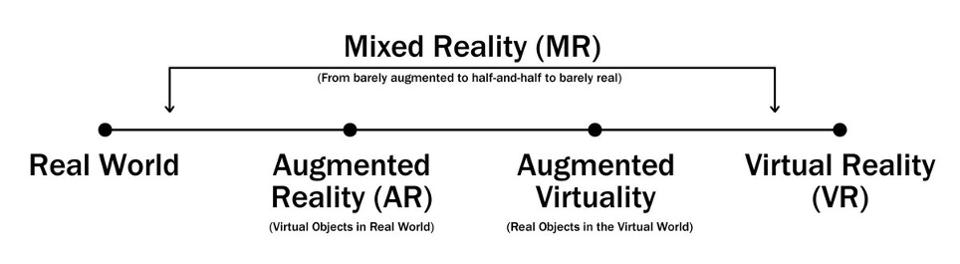
\includegraphics[width=\linewidth]{images/RealitySpectrum}
\caption{Représentation de continuum de la virtualité par Milgram et Kishino, 1995\cite{milgram1995augmented}}
\label{fig:realityspectrum}
\end{figure}

\paragraph{Réalité augmentée}
La réalité augmentée plus communément appelé \emph{Augmented Reality (AR)} quant a elle est un sous domaine de la réalité virtuelle. L'idée de la réalité augmentée est de venir superposer à l'environnement réel des éléments virtuels. Ces éléments vont alors venir "augmenter" notre monde en apportant le plus souvent des compléments d'informations. Elle est donc qualifié de sous domaine de la réalité virtuelle car l'utilisateur n'est plus immergé dans un environnement complètement numérique mais du contenu virtuel est ajouté en contexte à la vision réelle. Par abus de langage le terme de réalité augmentée est souvent utilisé pour parler de réalité mixte dont la notion est détaillé dans cette partie.
Il faut noter que ce type de réalité ne se base pas uniquement sur des \emph{HMD} mais peut être aussi apprécié à l'aide d'un téléphone par exemple (fig~\ref{fig:AR}).

\begin{figure}[H]
\centering
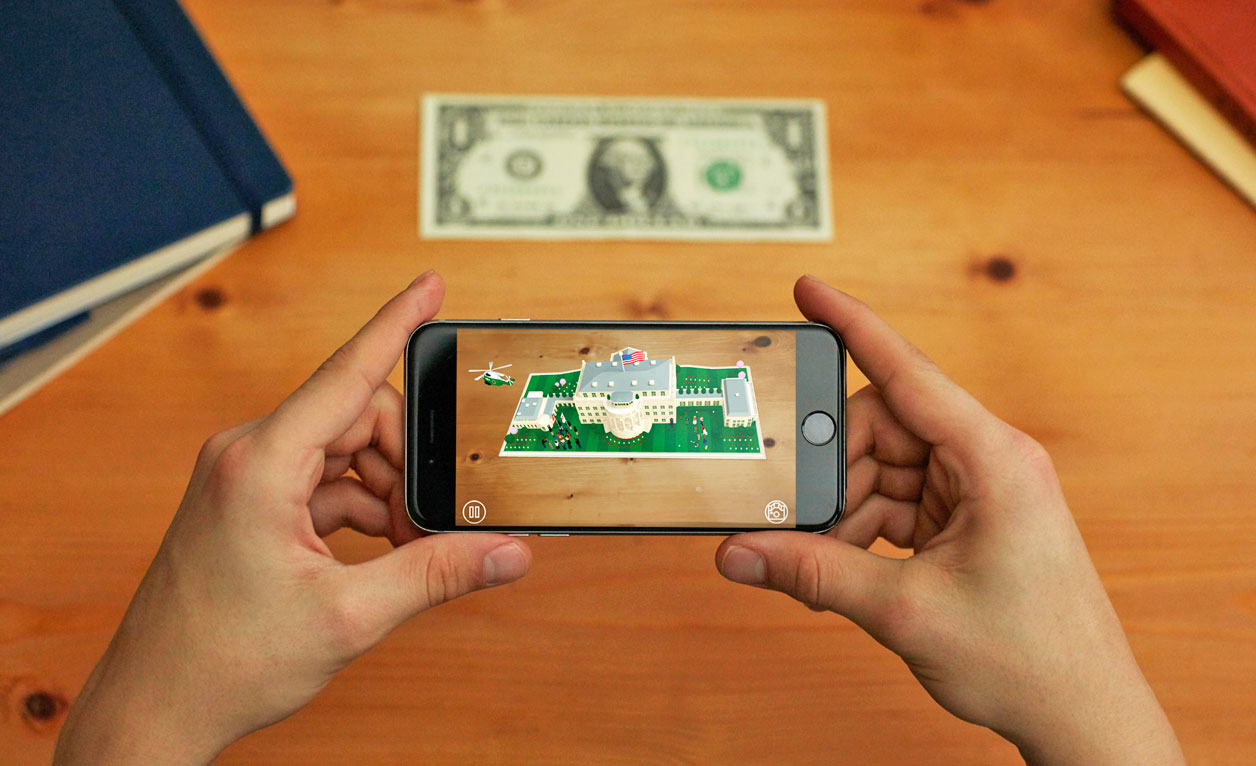
\includegraphics[width=0.55\textwidth]{images/AR}
\caption{Réalité augmentée vu au travers d'un téléphone\protect\footnotemark}\label{fig:AR}
\end{figure}
\footnotetext{Source: \href{https://www.engadget.com}{https://www.engadget.com}}

\paragraph{Réalité mixte}
La réalité mixte, ou hybride, plus communément appelé \emph{Mixed Reality (MR)}, ou \emph{Crossed Reality (XR)}, est la fusion parfaite de l'environnement numérique et de l'environnement physique (fig~\ref{fig:realityspectrum}). Dans ce "nouvel" environnement, les objets physiques et numériques coexistent et peuvent interagir entre eux et par exemple une table peut devenir une plateforme pour un personnage virtuel (fig~\ref{fig:youngconker}). Souvent confondu avec la réalité augmentée, cette dernière se différencie car elle ne propose pas seulement une visualisation des objets numériques, elle propose aussi des méthodes d'interactions avec ce contenu et c'est cette notion d'interaction qui permet de la différencier. A l'heure actuelle la réalité mixte nécessite un dispositif de type \emph{HMD} pour être appréciée comme par exemple  l'\texttt{HoloLens} de \texttt{Microsoft}.

\begin{figure}[H]
\centering
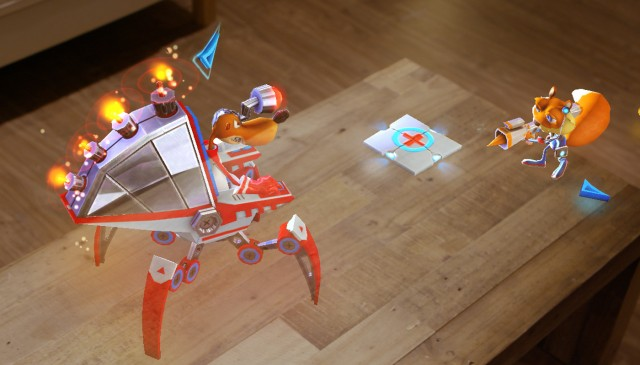
\includegraphics[scale=0.4]{images/youngconker}
\caption{Asobo Studio\texttrademark - Young Conker\copyright}
\label{fig:youngconker}
\end{figure}

\paragraph{Réalité augmentée vue au travers}
% Trouver qui l'a inventé et quand
La réalité augmentée vue au travers, plus communément appelé \emph{See Through Augmented Reality (STAR)} est une technique de visualisation de la réalité augmentée ou les éléments numériques sont vu au travers d'un écran (fig~\ref{sub:STARGO}) ou d'un \emph{HMD} (fig~\ref{sub:STARHolo}). C'est le type de visualisation le plus  utilisé actuellement. L'un des défauts majeur de ce type de visualisation est que la plus part du temps, chaque utilisateur a besoin de son propre écran ou casque pour pouvoir en profiter pleinement ce qui limite grandement les expériences collaboratives. Aussi les principaux défauts liés aux écrans s'appliquent aussi, a savoir fatigue visuel etc.  

\begin{figure}[H]
    \centering
	\subfloat[Pokémon GO - Vue au travers téléphone\protect\footnotemark]{
      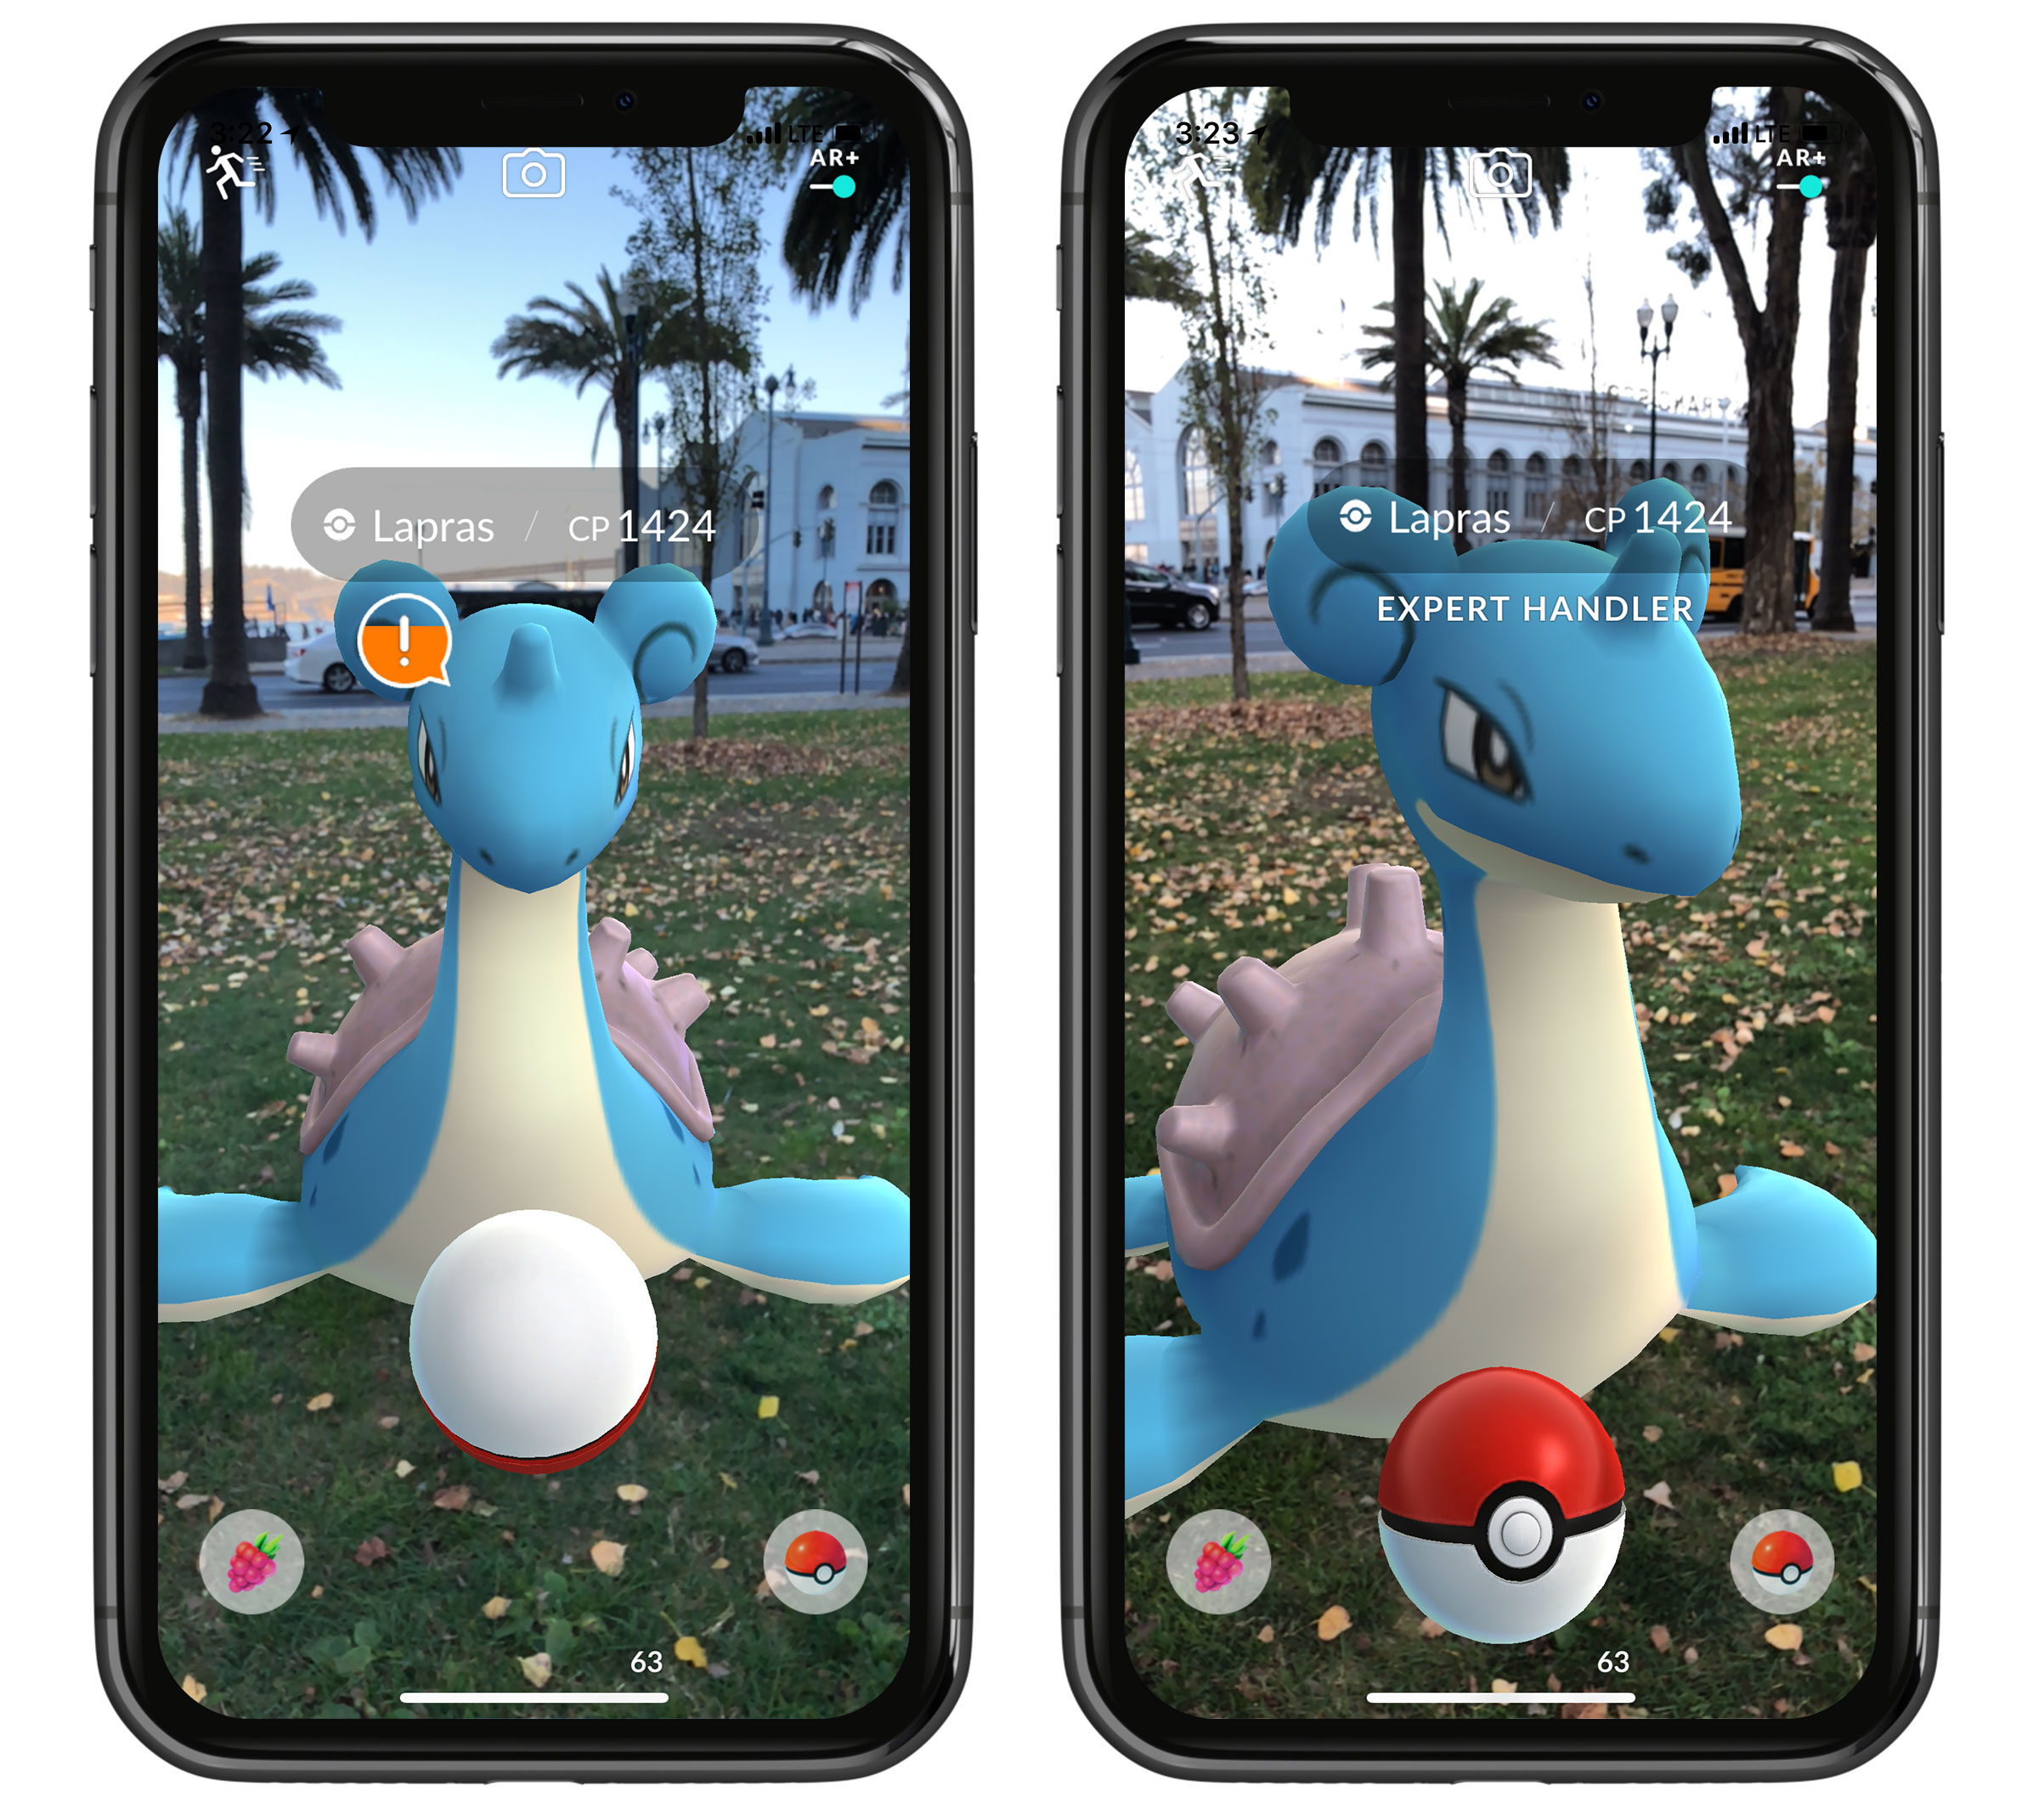
\includegraphics[width=0.45\textwidth]{images/pokemongo}
      \label{sub:STARGO}
      }
    \subfloat[Microsoft HoloLens - Vue au travers casque\protect\footnotemark]{
      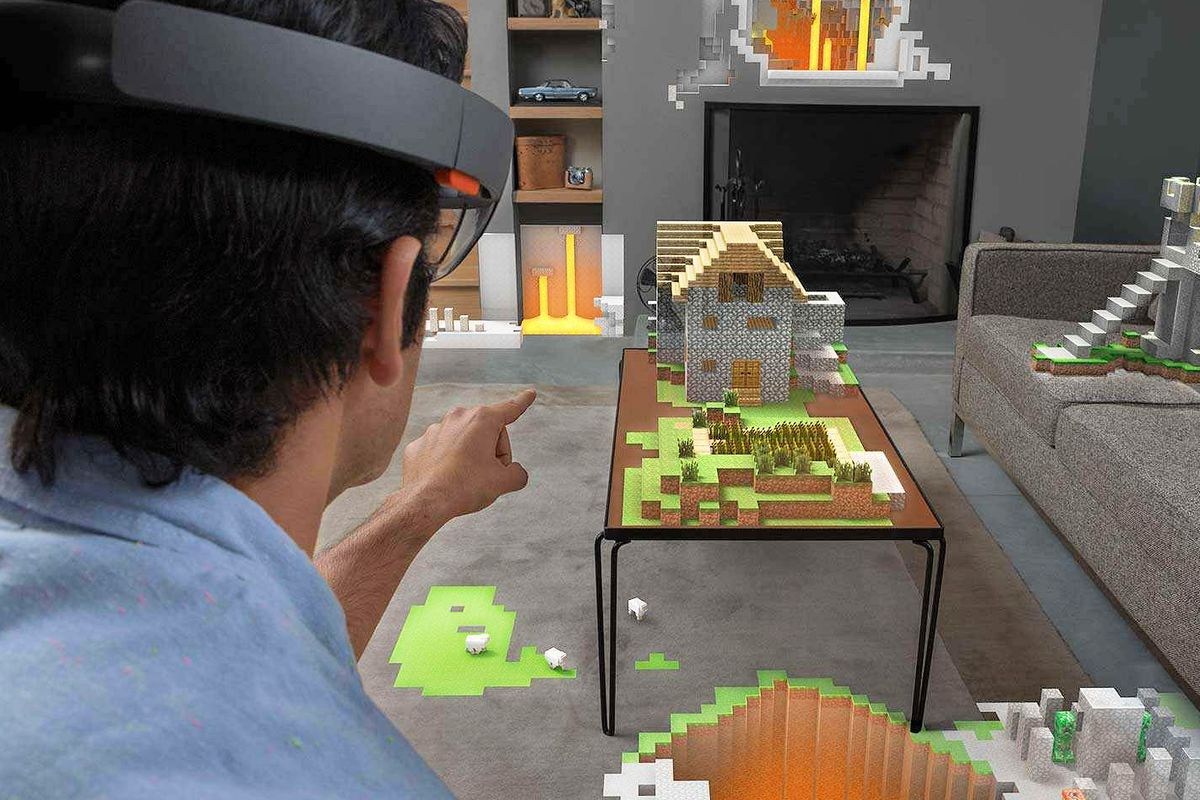
\includegraphics[width=0.45\textwidth]{images/hololens}
      \label{sub:STARHolo}
      }
\caption{Réalité augmentée vue au travers}
\label{fig:STAR}
\end{figure}
\footnotetext{Source: \href{https://pokemongolive.com/fr/}{Pokemon GO}}
\footnotetext{Source: \href{https://www.microsoft.com/fr-fr/hololens}{Microsoft HoloLens}}

\paragraph{Réalité augmentée spatiale}
% Trouver qui l'a inventé et quand
La réalité augmentée spatiale, plus communément appelé \emph{Spatial Augmented Reality (SAR)} est une technique de visualisation de la réalité augmentée se basant sur un dispositif de projection. Les éléments virtuels qui viennent "augmenter" le monde réel sont alors projetés dans l'espace (fig~\ref{fig:SAR}), d'où le terme spatiale. Cette notion d'augmentation de l'espace tend à rendre cette technologie naturellement collaborative car les projections ne dépendent pas d'un dispositif visuel personnel et sont obligatoirement partagées. La SAR permet aussi de favoriser le développement d'interface tangible, en effet, la visualisation se faisant directement sur les objets physiques, la tendance à développer des interfaces en communion avec ceux ci est très forte car très naturel.

\begin{figure}[H]
\centering
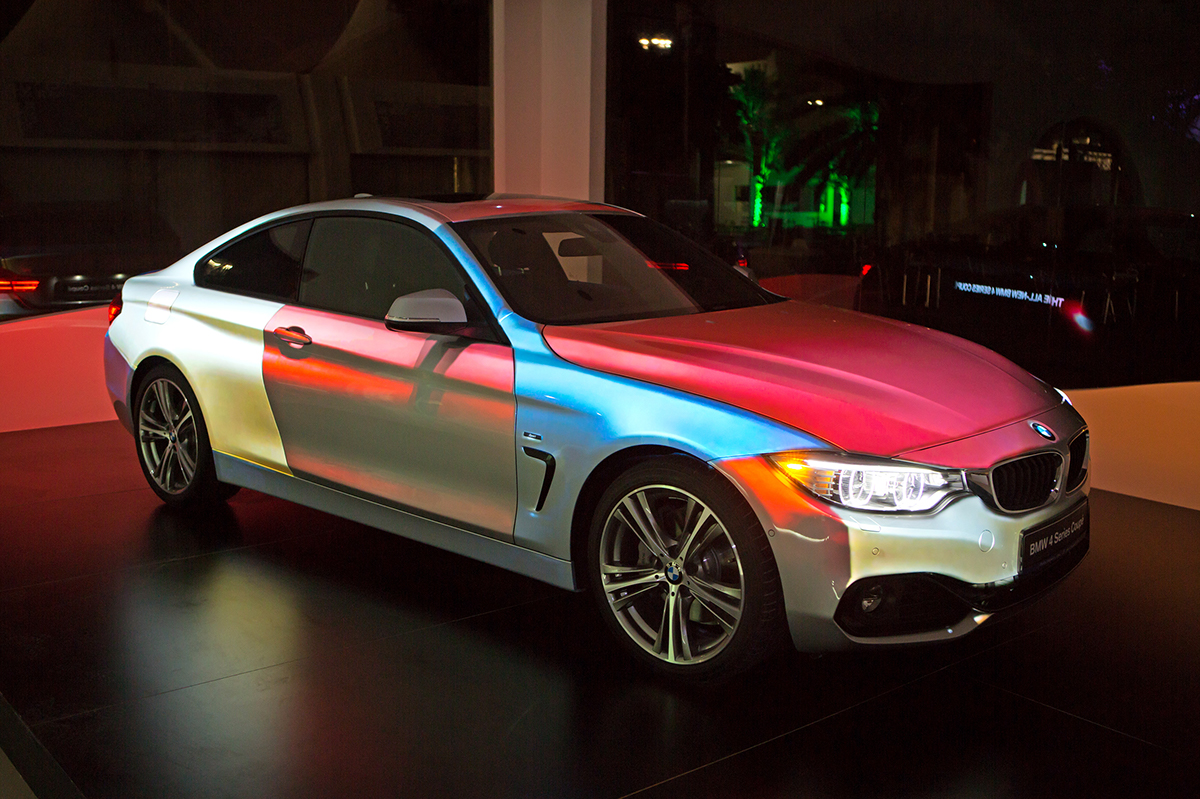
\includegraphics[width=0.5\textwidth]{images/SARMappingCar2}
\caption{Présentation d'une voiture en utilisant de la réalité augmentée spatiale\protect\footnotemark}
\label{fig:SAR}
\end{figure}
\footnotetext{Source: {Google Image}}

\paragraph{Interface tangible}
Une interface utilisateur tangible ou \emph{Tangible User Interface (TUI)} est une interface utilisateur via laquelle des objets physiques, ou encore le toucher, permettent de manipuler des données numériques (fig~\ref{sub:TUI}). Les interfaces utilisateurs tangibles remplacent très souvent les interfaces utilisateur graphiques (fig~\ref{sub:GUI}) où \emph{Graphical User Interface (GUI)} dans la plupart des application de réalité augmentée car elles fournissent un contrôle direct à l'utilisateur sur ce qu'il souhaite manipuler (par opposition au contrôle indirect, comme la souris, nécessaire à la manipulation des GUI).

\begin{figure}[H]
    \centering
	\subfloat[Interface Utilisateur Graphique (GUI)\protect\footnotemark]{
      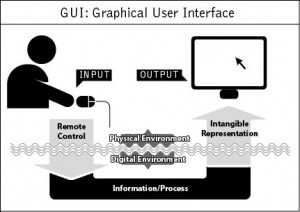
\includegraphics[width=0.45\textwidth]{images/GUI}
      \label{sub:GUI}
      }
    \subfloat[Interface Utilisateur Tangible (TUI)\protect\footnotemark]{
      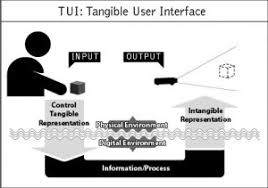
\includegraphics[width=0.45\textwidth]{images/TUI}
      \label{sub:TUI}
      }
\caption{Différences des interfaces utilisateurs}
\label{fig:GUITUI}
\end{figure}
\footnotetext{Source: \href{http://iconlibrary.iconshock.com/design/from-gui-to-tui/}{Icon Library - From GUI to TUI}}
\footnotetext{Source: \href{http://iconlibrary.iconshock.com/design/from-gui-to-tui/}{Icon Library - From GUI to TUI}}

\paragraph{Calcul haute performance}
Le calcul haute performance ou \emph{General-Purpose computing on Graphics Processing Units (GPGPU)} désigne une méthode de calcul utilisant la carte graphique (GPU) plutôt que le processeur (CPU). Cette technique permet de bénéficier de la puissance de la carte graphique afin de réaliser du calcul en parallèle et est très souvent utilisée pour la plupart des traitement lourd comme par exemple le rendu d'une scène 3D, l'encodage de vidéo, les simulations physiques (particules) etc. Cette technique repose sur le grand nombre de cœurs présent dans les cartes graphiques (contrairement aux processeurs) et sur la capacité de chacun de ces cœurs à effectué des opérations simples de manière très efficace. Le calcul haute performance ne peut cependant pas ce passer du CPU qui va être principalement utilisé pour récolter et transférer les données traités ou à traiter.
% Expliquer comment ca marche (carte graphique beaucoup de coeur pour faire des opérations simple, CPU pas beaucoup de coeur donc plus lent)
% Ajouter image comparaison

\begin{figure}[H]
\centering
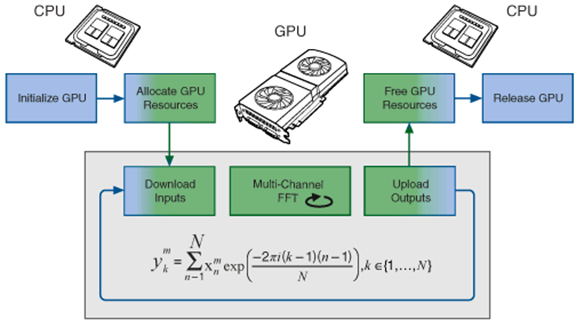
\includegraphics[scale=0.7]{images/gpuworkflow}
\caption{Exemple de calcul de la FFT sur GPU\protect\footnotemark}
\label{fig:gpgpu}
\end{figure}
\footnotetext{Source: \href{http://www.ni.com/white-paper/14077/fr/}{National Instruments}}


\chapter{État de l'art}

Intro

\section{PapARt}

\section{Système de réalité augmentée spatiale}

\section{Bilan}

\chapter{Développement d'application}

Comme présenté dans l'introduction (chapitre ~\ref{chap:intro}), le premier objectif du stage était le développement d'applications de réalité augmentée spatiale. Il était important, pour commencer, d'évaluer les possibilités mais aussi les contraintes qu'offrait le kit de développement. 
Ainsi, un travail d'analyse et de critique de l'interface de programmation (\emph{Application Programming Language API}) à été effectué en parallèle du développement d'applications.

\section{ReARTable}
\label{sec:reartable}
En tenant compte du contexte et du public ciblé par l'entreprise, il m'a paru intéressant de développer une démonstration dont le but était à la fois ludique et éducatif. J'ai donc choisi de recréer une Reactable\cite{reactable}, proposée par la société du même nom, en réalité augmentée spatiale, que nous avons nommé ReARTable.

La Reactable est un instrument de musique électronique permettant la génération de sons en direct, développé depuis 2003. Présenté sous la forme d'une table interactive, le son est généré via des éléments tangibles placés à sa surface Figure~\ref{fig:reactelem}. 

\begin{figure}[H]
\centering
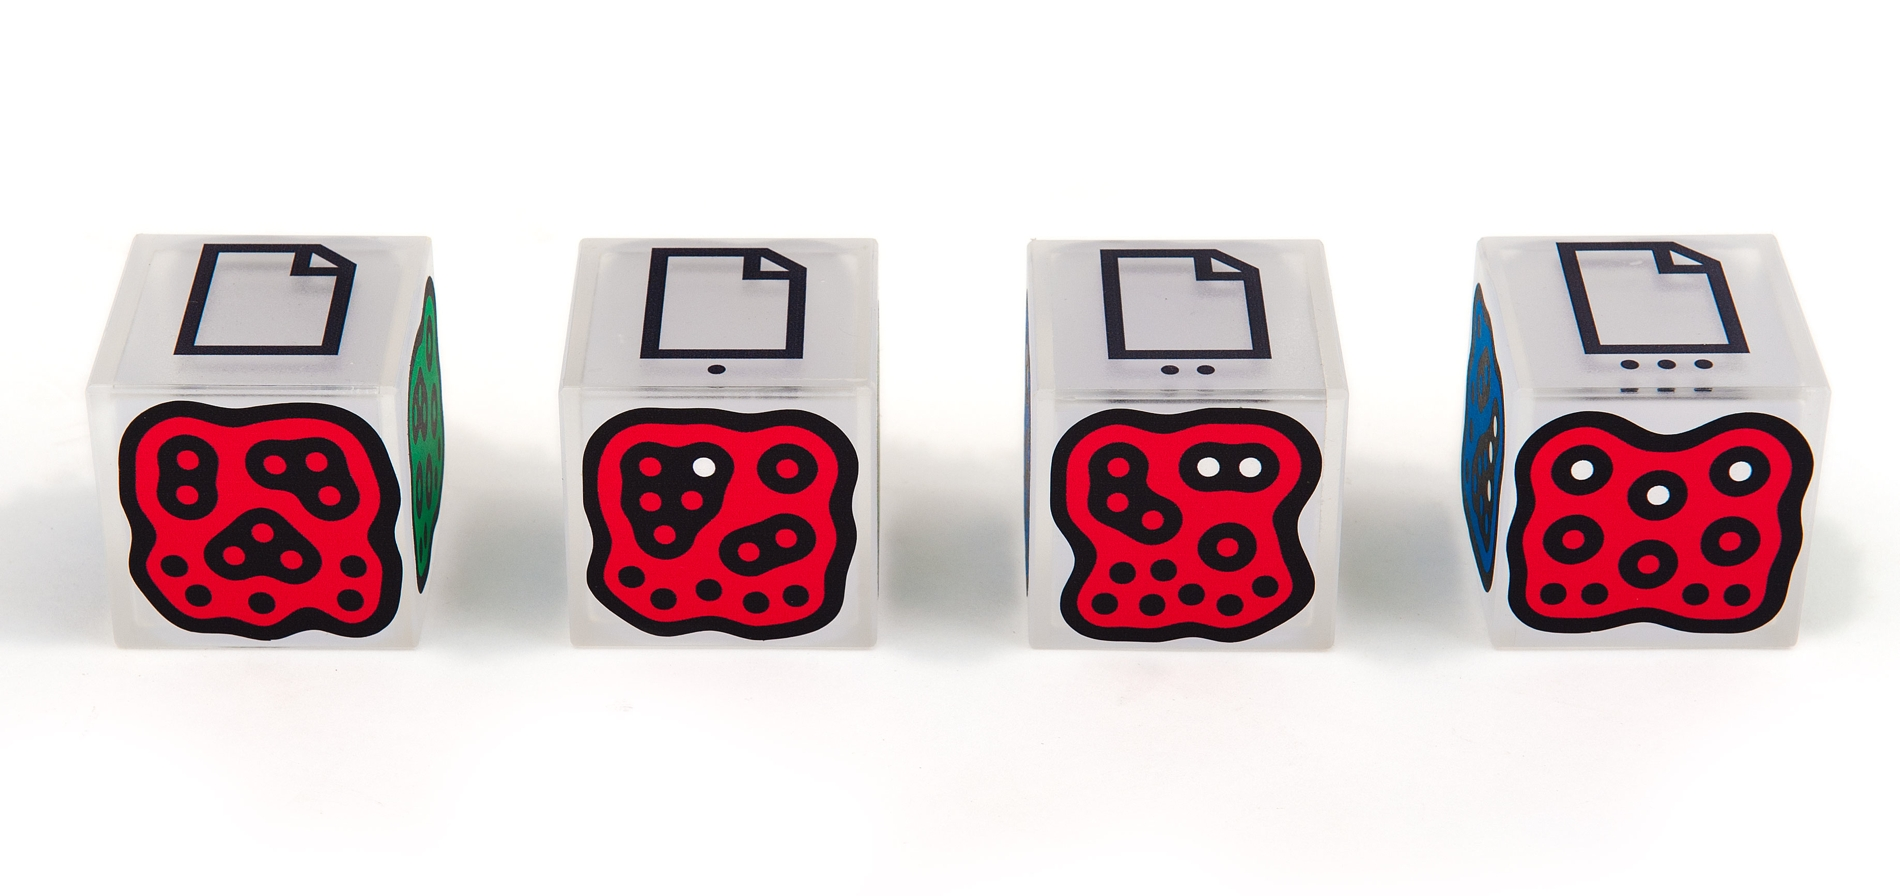
\includegraphics[width=0.6\textwidth]{images/reactelements}
\caption{Éléments tangibles utilisés pour la génération d'un élément de synthétiseur sur la Reactable\protect\footnotemark}
\label{fig:reactelem}
\end{figure}

\footnotetext{Source: \href{http://a-blok.com/FR/reactable.html}{Reactable : Elements tangibles}}

Chaque élément tangible représente un élément de synthétiseur qu'il est possible de contrôler de plusieurs façons:
\begin{itemize} 
\item La distance de l'élément par rapport à un autre élément. Cette propriété peut être utilisée pour contrôler, par exemple, l'interaction entre deux éléments.
\item L'orientation de l'élément sur la table. Cette propriété peut être utilisée pour contrôler, par exemple, la fréquence de l'élément ce qui va avoir pour effet si l'on prend l'exemple d'un battement de ralentir ou d'accélérer ce dernier.
\item La disposition de l'élément. Cette propriété permet, entre autres, de combiner des éléments pour créer de nouveaux sons, plus riches et plus complexes.
\item La position du doigt de l'utilisateur par rapport à un élément. On peut venir contrôler divers paramètres comme l'amplitude par exemple, en faisant graviter son doigt autour d'un élément.
\end{itemize}
Ainsi, c'est en combinant plusieurs éléments entre eux avec différentes orientations et différentes dispositions que l'utilisateur va pouvoir peu à peu "construire" sa musique.
Au-delà de la détection des éléments tangibles, la table est rétro éclairée et permet donc la visualisation, en direct, de la musique générée Figure~\ref{fig:reactivsu}.

\begin{figure}[H]
\centering
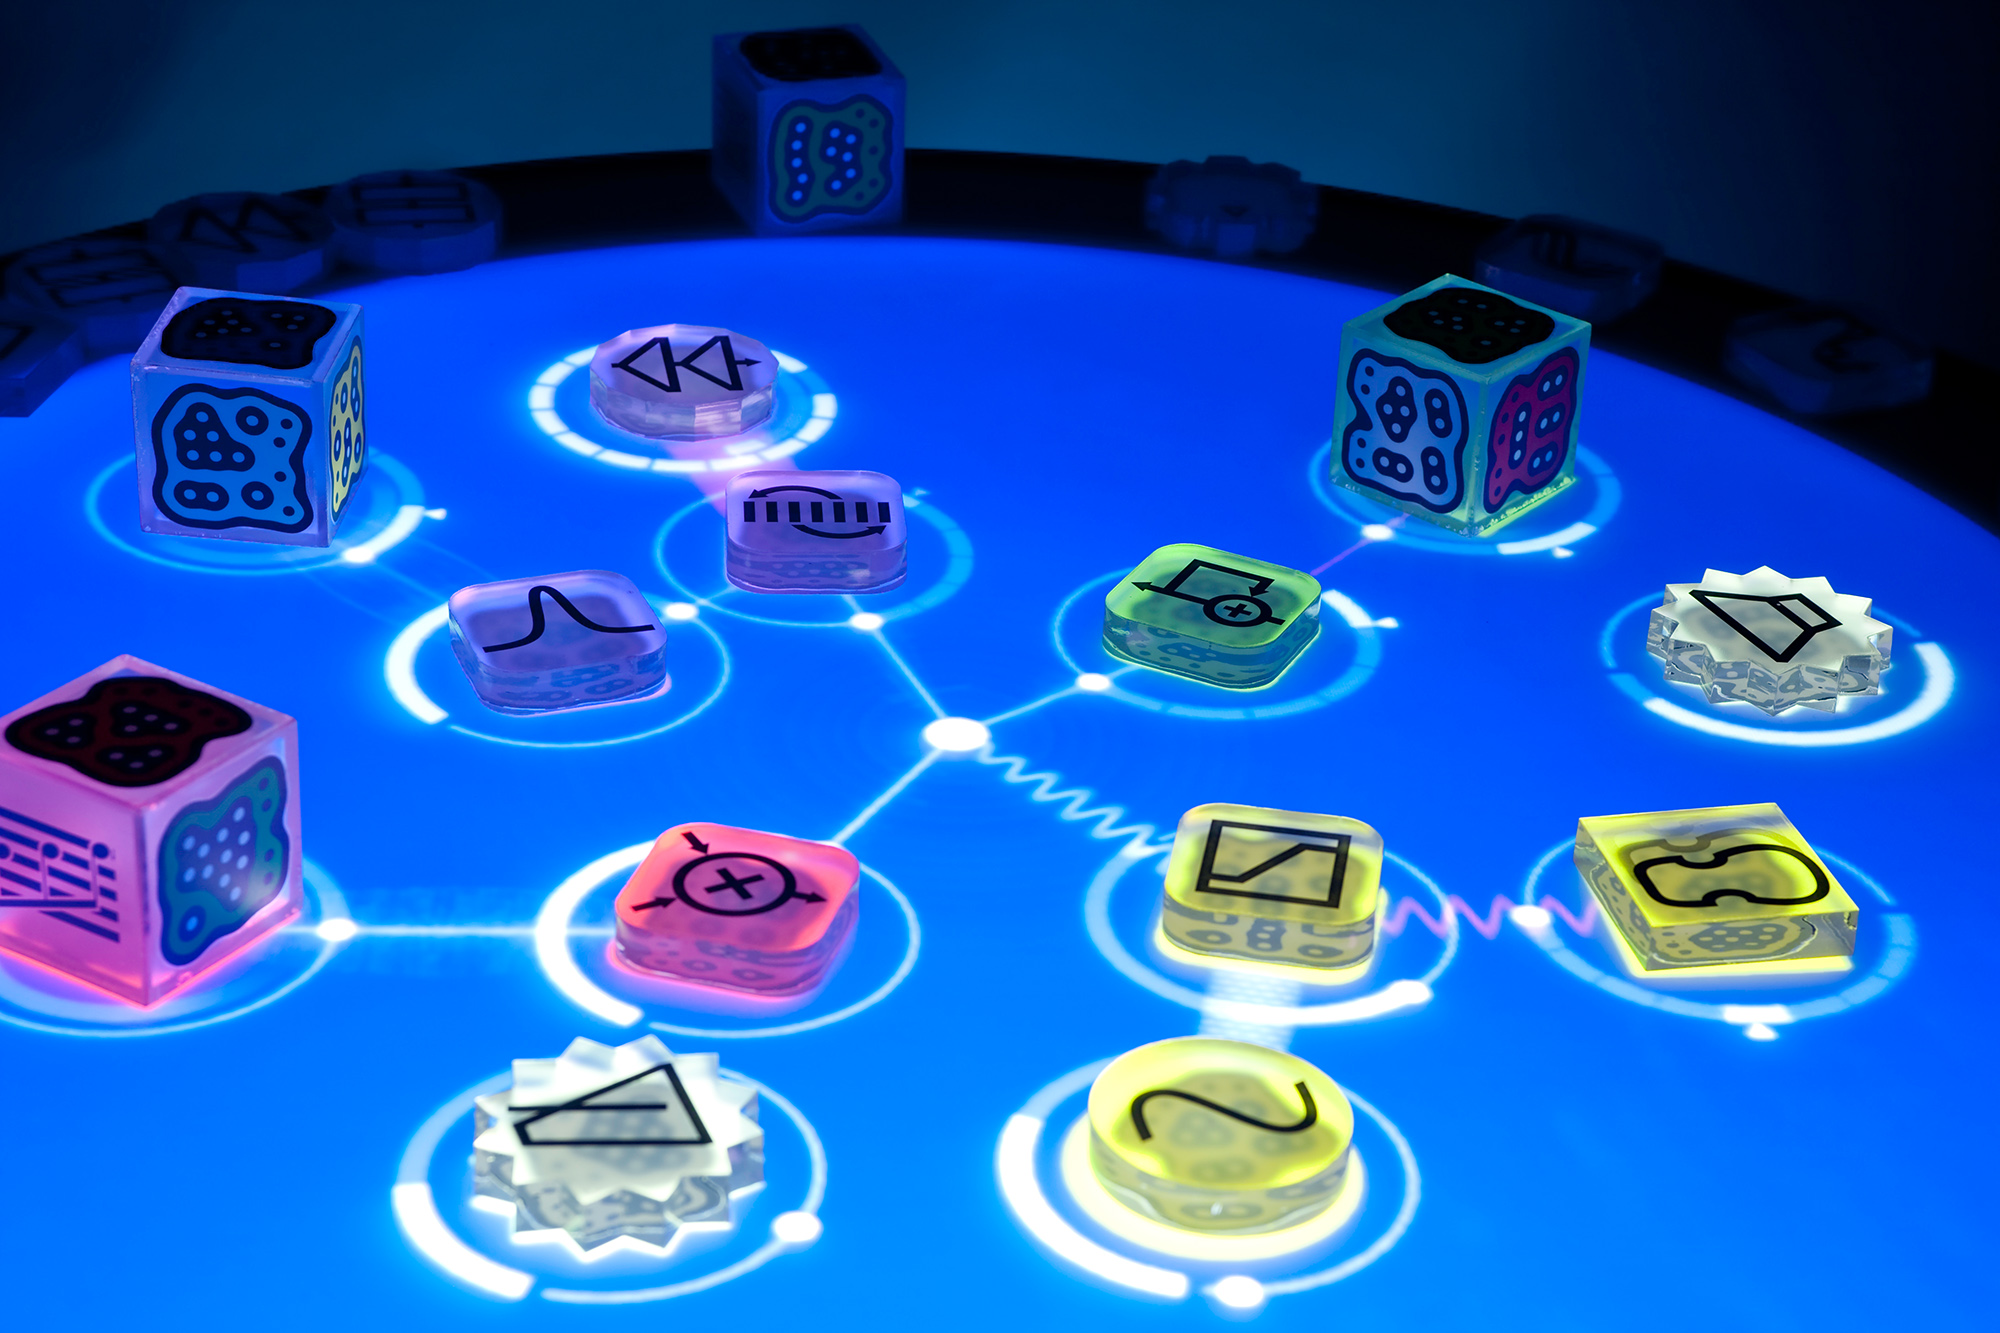
\includegraphics[width=0.65\textwidth]{images/reactvisu}
\caption{Visualisation du son sur la Reactable\protect\footnotemark}
\label{fig:reactivsu}
\end{figure}

\footnotetext{Source: \href{http://a-blok.com/FR/reactable.html}{Reactable}}

\subsection{Besoins de l'application}
\label{subsec:reartable:content}
Le but de l'application était de présenter une démonstration de ce qu'est capable de faire le système proposé par RealityTech, et non de créer un simulateur de musique en direct, finit, reprenant tous les points de la Reactable. Un tel développement pourrait faire l'objet d'un stage entier, ce qui n'était pas le cas ici.\\

Pour être en adéquation avec l'idéologie de l'entreprise, l'interface tangible ainsi que les modes d'interaction avec la musique étaient les points les plus importants à considérer. En gardant cela à l'esprit, nous avons défini les besoins fonctionnels principaux que voici :
\begin{itemize}
\item Générer du son en direct.
\item Créer une représentation physique du son. Chaque son ou élément sonore devait avoir une représentation physique qui lui était associée, c'est à dire, un élément ou groupement d'éléments tangibles le représentant.
\item Détecter des éléments physiques représentant les éléments sonores dans une image. L'application devait pouvoir détecter dans une image de caméra les divers éléments physiques présents, de façon à ce qu'ils soient utilisés pour identifier les éléments sonores.
\item Identifier les représentations des sons. Chaque élément sonore étant représenté par un ou plusieurs éléments physiques, l'application devait être capable, à partir des résultats de la détection, d'identifier et de différencier des éléments sonores entre eux. 
\item Modifier un élément sonore. L'application devait pouvoir contrôler certains paramètres définis à l'avance de chaque élément sonore généré. Ces paramètres ont pour but d'apporter à l'utilisateur un niveau de contrôle supérieur lors de la création de musique en direct.
\item Détecter des événements liés au toucher. Dans le cas du contrôle d'un son, l'utilisateur peut être amené à toucher des zones interactives pour déclencher divers effets.
\item Créer une visualisation basique d'un son. L'application devait proposer une visualisation du son généré, pour guider l'utilisateur dans son expérimentation.
\end{itemize}

\subsection{Choix et implémentation}
\label{subsec:reartable:impl}
L'application a donc été développée avec Processing, en utilisant, d'une part, PapARt pour la partie visualisation, détection et projection et, d'autre part, Sonic Pi\cite{sonicpi} pour la génération de musique en direct.
Sonic Pi est un synthétiseur temps réel qui permet de générer très facilement des sons de manière cohérente. Le gros avantage de Sonic Pi est qu'il résout tout seul bon nombre de problèmes posés par la génération dynamique de musique comme, par exemple, la synchronisation des boucles, les effets d'entrée et de sortie des instruments et bien d'autres, ce qui dé-complexifie énormément le processus.

Comme on peut le voir sur le schéma explicatif ci-dessous Figure~\ref{fig:reartable:generalscheme}, les éléments tangibles représentant des sons apparaissent sous forme de regroupement d'éléments ronds de petite taille (des aimants dans notre cas). L'idée derrière ce choix est d'encourager la manipulation d'éléments physiques pour garder le contenu numérique en contexte et ainsi favoriser la création. On peut différencier deux sons en fonction du contenu du regroupement (nombre, position et couleur des éléments regroupés).

\begin{figure}[H]
\centering
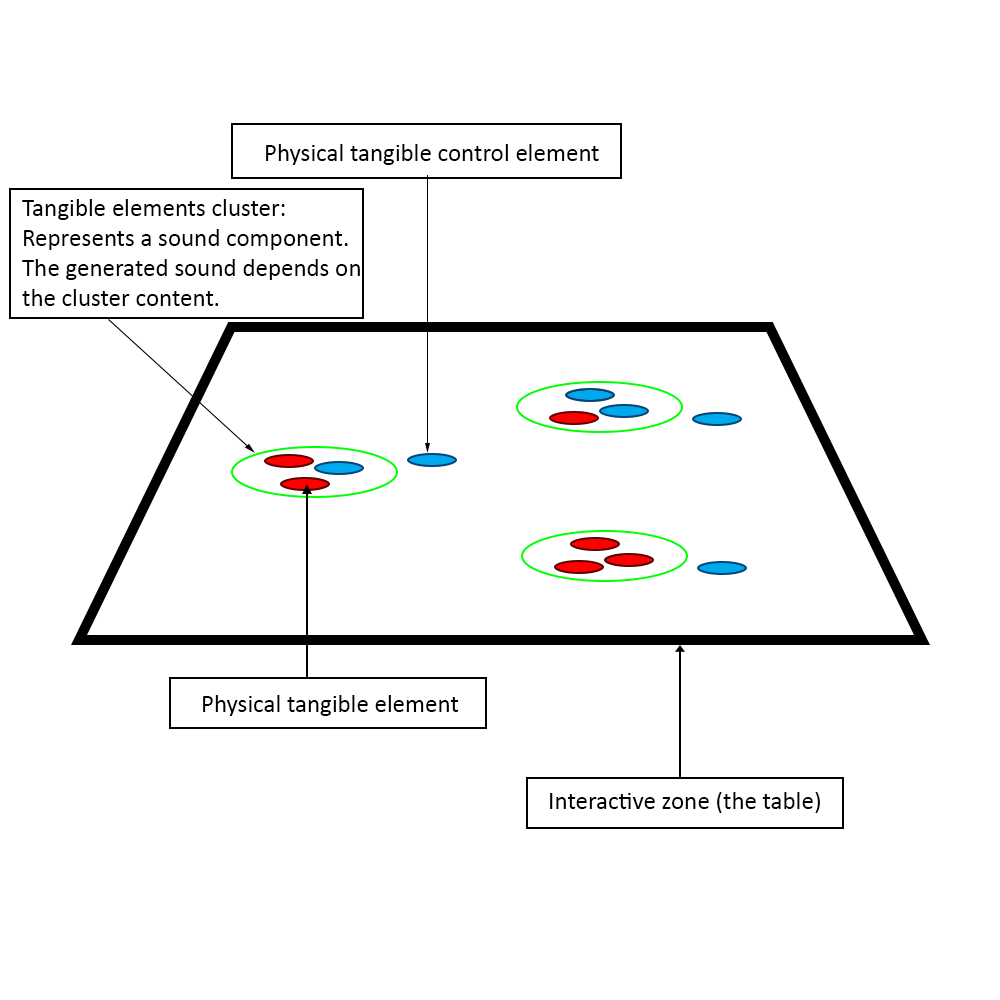
\includegraphics[width=0.5\linewidth]{images/rearproto}
\caption{ReARTable: Illustration du concept}
\label{fig:reartable:generalscheme}
\end{figure}

Une fois les éléments détectés, regroupés et identifiés, l'élément sonore associé peut être créé. La création de l'élément sonore se fait simplement via la transmission d'un message OSC\footnote{Le protocole OSC ou OpenSoundControl est un format de transmission de donnée conçu pour le contrôle en temps réel} à un serveur Sonic Pi préalablement démarré. Ce message contient l'identifiant unique de la boucle que Sonic Pi doit démarrer. Pour chaque élément sonore que l'application peut créer, Sonic Pi possède une fonction à exécuter que nous avons préalablement créée. Toutes les communications entre l'application et Sonic Pi utilisent ce protocole ce qui permet de démarrer/arrêter/modifier certaines parties du son en direct.

Pour ce qui est du contrôle du son, une zone autour du composant est définie dans laquelle soit un élément tangible, soit une interaction physique (avec le doigt) vont être détectés et convertis en interaction avec le contenu numérique Figure~\ref{fig:reartable:interactionzone}.

\begin{figure}[H]
\centering
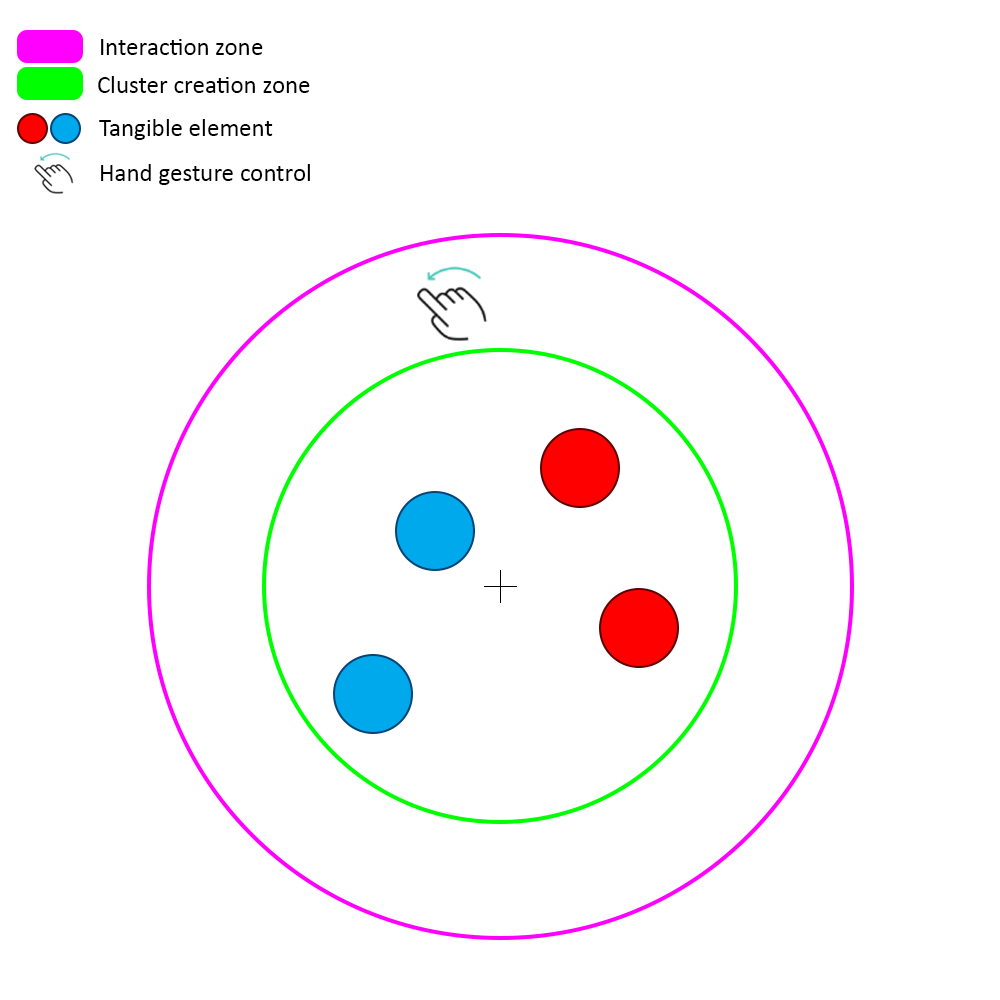
\includegraphics[width=0.45\textwidth]{images/reartable_cluster_interaction}
\caption{Schéma représentant la création d'un son avec zone d'interaction}
\label{fig:reartable:interactionzone}
\end{figure}

La dernière étape du développement de l'application concernait la visualisation de la musique générée section~\ref{subsec:reartable:content}. Cette étape n'a finalement pas été aboutie par manque de temps. L'idée était d'utiliser le spectre du son et les différentes fréquences qui le compose, récupérables à l'aide d'une transformée de Fourier\footnote{Opération mathématique permettant de décomposer un signal en la somme des signaux qui le compose \href{https://fr.wikipedia.org/wiki/Transformation_de_Fourier}{Wikipédia - Transformation de Fourier}.}, pour créer une visualisation globale basée sur les fréquences avec des variations visuelles en fonction de la hauteur, du tempo et de tous les autres paramètres du son qu'il est possible d'extraire et d'utiliser.\\

Vous trouverez Figure~\ref{fig:reartable:demo} un aperçu de l'état actuel de l'application. 

\begin{figure}[H]
\centering
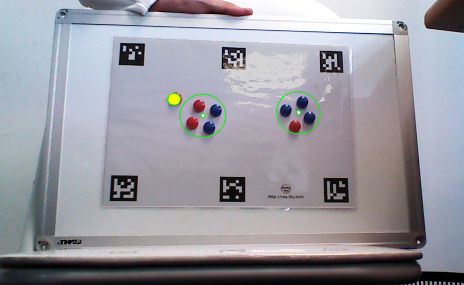
\includegraphics[width=0.65\linewidth]{images/reartable}
\caption{Démonstration de l'application}
\label{fig:reartable:demo}
\end{figure}

\newpage
\section{Extraction de document}
\label{sec:document}
Plus tard au cours de mon stage, nous avons eu l'occasion d'aborder des problématiques comme l'extraction et la numérisation de document (par exemple dans le cas de l'écriture d'une lettre en réalité augmentée) en tant que cas d'utilisation de PapARt. Il était donc opportun de développer une preuve de concept de cette fonctionnalité sous la forme d'une application de réalité augmentée spatiale.

Le but de ce développement était d'expérimenter diverses techniques de détection de document en temps réel, se basant ou non sur des connaissances à priori comme la taille du document, sa couleur, la couleur du fond (duquel il faudrait extraire le document), la présence d'éléments distinctifs (tels que des marqueurs fiduciaires ou des ronds colorés de petite taille) etc.

\subsection{Besoins de l'application}
\label{subsec:doc:content}
\begin{itemize}
\item Accéder au flux vidéo d'une caméra. L'application devait avoir access au flux vidéo d'une caméra filmant le document à détecter.
\item Détecter un document dans une image. Des images extraites du flux vidéo, l'application devait être capable, avec ou sans connaissance a priori, de détecter un document se trouvant dans cette image.
\item Extraire un document d'une image. Grâce au résultat de la détection, l'application devait être capable d'extraire ce document de l'image afin d'obtenir une image ne contenant que le dit document.
\end{itemize}

\subsection{Choix et implémentation}
\label{subsec:doc:impl}

La détection de document est un problème connu en traitement d'image, sur lequel j'avais déjà eu l'occasion de travailler lors de mon projet de fin d'études durant le deuxième semestre de mon année de Master 2.

Dans cette application, nous donc avons explorer plusieurs solutions sollicitant différents procédés dans le but d'essayer de trouver une solution adéquate à ce problème.

\subsubsection{Détection de document basée sur des marqueurs colorés} Le premier prototype de détection que nous avons conçu utilise beaucoup de connaissances à priori sur le document afin de faciliter la détection. Ainsi, le document cible est muni de lignes d'éléments ronds, colorés, de petite taille, dans un ou plusieurs de ses coins (fig~\ref{sub:doc}). Les éléments ronds de petite taille sont détectés grâce à PapARt en réalisant une convolution de l'image par un filtre permettant la détection de ces derniers dont le principe détaillé section~\ref{ssec:convtheo}.

Une fois les éléments détectés, ils sont regroupés en différentes lignes (fig~\ref{sub:docline}).
Une ligne est définie par un regroupement d'éléments dont l'écart entre chaque élément ne dépasse pas une certaine distance verticale ou horizontale. L'angle de la ligne est défini par les $x$ premiers éléments qui la compose, $x$ étant le nombre minimum d'éléments composant une ligne (fig~\ref{fig:doc:linecluster}). Si un autre élément "dérive" il est rejeté et la ligne est créée. Cette ligne est ensuite utilisée pour calculer deux vecteurs, dont un est confondu avec la ligne et le deuxième est perpendiculaire au premier (fig~\ref{sub:doclineperp}).

La détection finale du document se fait en calculant l'intersection des différents vecteurs verticaux et horizontaux (fig~\ref{sub:docextract})

\begin{figure}[H]
    \centering
	\subfloat[Document marqué à détecter]{
      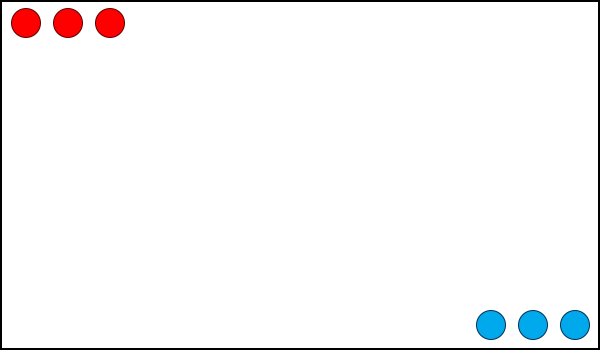
\includegraphics[width=0.45\textwidth]{images/document}
      \label{sub:doc}
      }
    \subfloat[Détection des éléments rond et création des lignes]{
      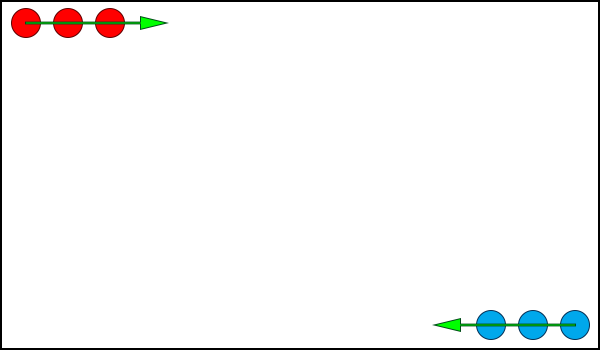
\includegraphics[width=0.45\textwidth]{images/doc-line}
      \label{sub:docline}
      }
      \\
      \subfloat[Génération des information manquante pour finaliser la détection]{
      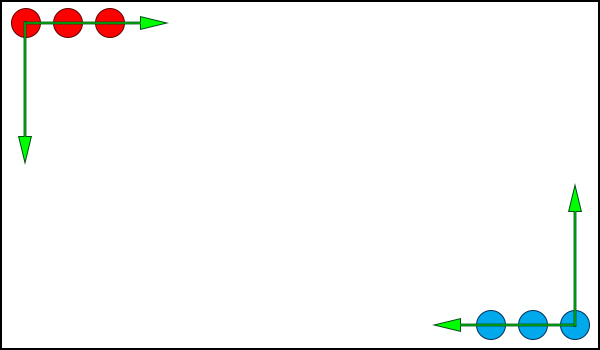
\includegraphics[width=0.45\textwidth]{images/doc-line-perp}
      \label{sub:doclineperp}
      }
    \subfloat[Document détecté]{
      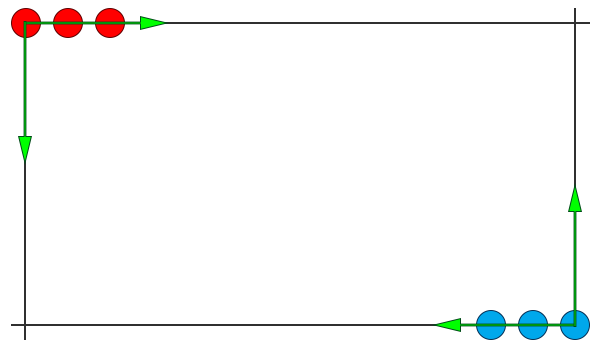
\includegraphics[width=0.45\textwidth]{images/doc-extraction}
      \label{sub:docextract}
      }
\caption{Détection de document étape par étape}
\label{fig:docdetection}
\end{figure}
	
\begin{figure}[H]
\centering
	\subfloat[]{
      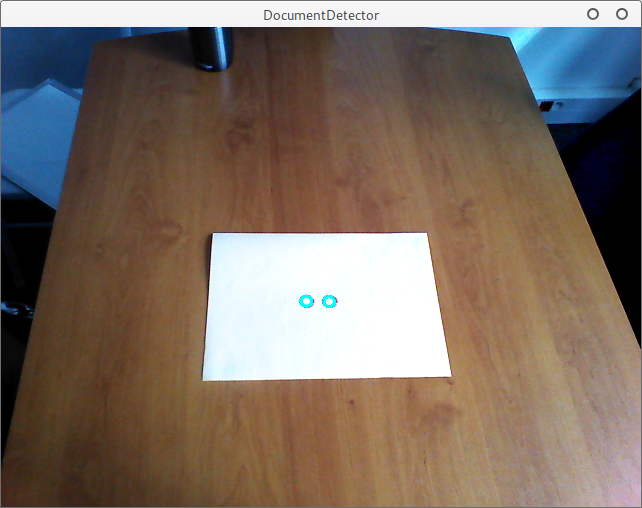
\includegraphics[width=0.45\textwidth]{images/document-detection-noline}
      \label{sub:doc:noline}
      }
      \subfloat[]{
      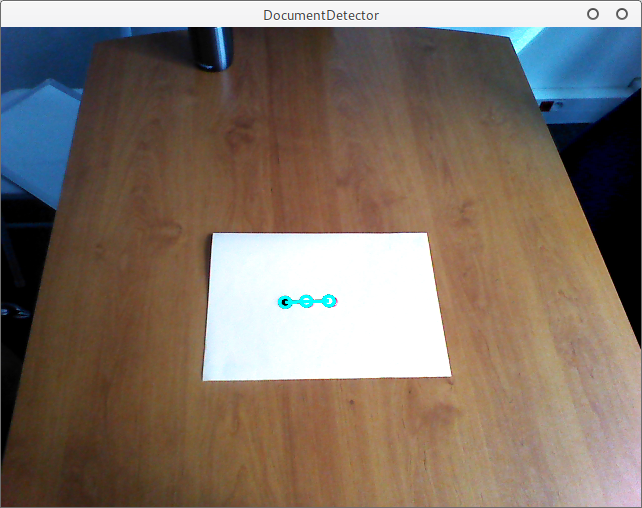
\includegraphics[width=0.45\textwidth]{images/document-detection-line}
      \label{sub:doc:line}
      }
      \caption{Détection et création d'une ligne a partir d'éléments colorés ($x = 3$)}
      \label{fig:doc:linecluster}
\end{figure}

Comme on peut le voir sur la figure ~\ref{sub:docextract}, lors de cette détection, les bords du document sont rognés. Généralement ces zones ne contiennent aucune information car elles correspondent le plus souvent aux marges verticales et horizontales présentes dans la plupart des documents. Cependant, comme évoqué dans les cas d'utilisation, cette détection ne sera pas seulement utilisée pour des documents de type A4, on pourra s'en servir comme outil pour suivre une feuille de papier à la manière des marqueurs \texttt{ARToolKitPlus}, ou pour détecter des post-it par exemple. Ainsi, ces marges ne peuvent pas être ignorées car elle sont susceptibles de contenir du contenu critique du document.

Une simple connaissance à priori de la distance des éléments ronds par rapport au coin permet de résoudre ce problème. Toutefois, si l'on souhaite obtenir une détection plus précise, il est conseiller d'utiliser des algorithmes de détection de contour couplés à des algorithmes d'extraction de lignes qui permettrons de retrouver de façon plus fidèle le coin du document. Cette re détection du coin est détaillée section~\ref{subsubsec:cannyhough}.

\subsubsection{Détection de document - Canny et transformée de Hough}
\label{subsubsec:cannyhough} 
Avec peu ou pas de connaissance a priori, la détection de document devient un problème compliqué et bien connu dans le domaine du traitement d'image surtout lorsqu'un besoin de temps réel vient s'ajouter à la tâche.

L'algorithme de Canny\cite{Canny86acomputational} est un filtre de détection de contours, permettant d'extraire d'une image (fig~\ref{sub:originalimage}) des contours très précis (fig ~\ref{sub:detectedge}) respectant trois critères : La bonne détection, la bonne localisation et la clarté de la réponse. Ces trois critères en font un très bon choix dans le cadre de la détection de document, où la qualité et surtout la précision de la détection est importante pour ne pas rogner des bouts de document par exemple. Cet algorithme a cependant tendance à laisser beaucoup de bruit issu de faibles contours tout de même détectés. C'est pourquoi il faut effectuer une étape de floutage préalable afin de lisser les zones à faibles contours.

Une fois les contours détectés, il est possible d'essayer d'extraire directement le document mais c'est une tâche complexe car elle requiert d'analyser les contours. Cette action peut être facilitée en utilisant une technique appelée transformée de Hough\cite{hough}. En effet, la transformée de Hough permet d'extraire n'importe quelle forme à partir d'une image contour en utilisant les propriétés mathématiques de celle ci. Dans notre cas, où nous souhaitons extraire des lignes droites, les propriétés mathématiques utilisées correspondent aux coordonnées polaires considérées comme plus robuste que l’équation de la droite (fig ~\ref{sub:detectline}). Il ne reste qu'à filtrer les lignes afin de trouver des potentiels documents dans une image.

\begin{figure}[H]
\centering
	\subfloat[Image originale]{
      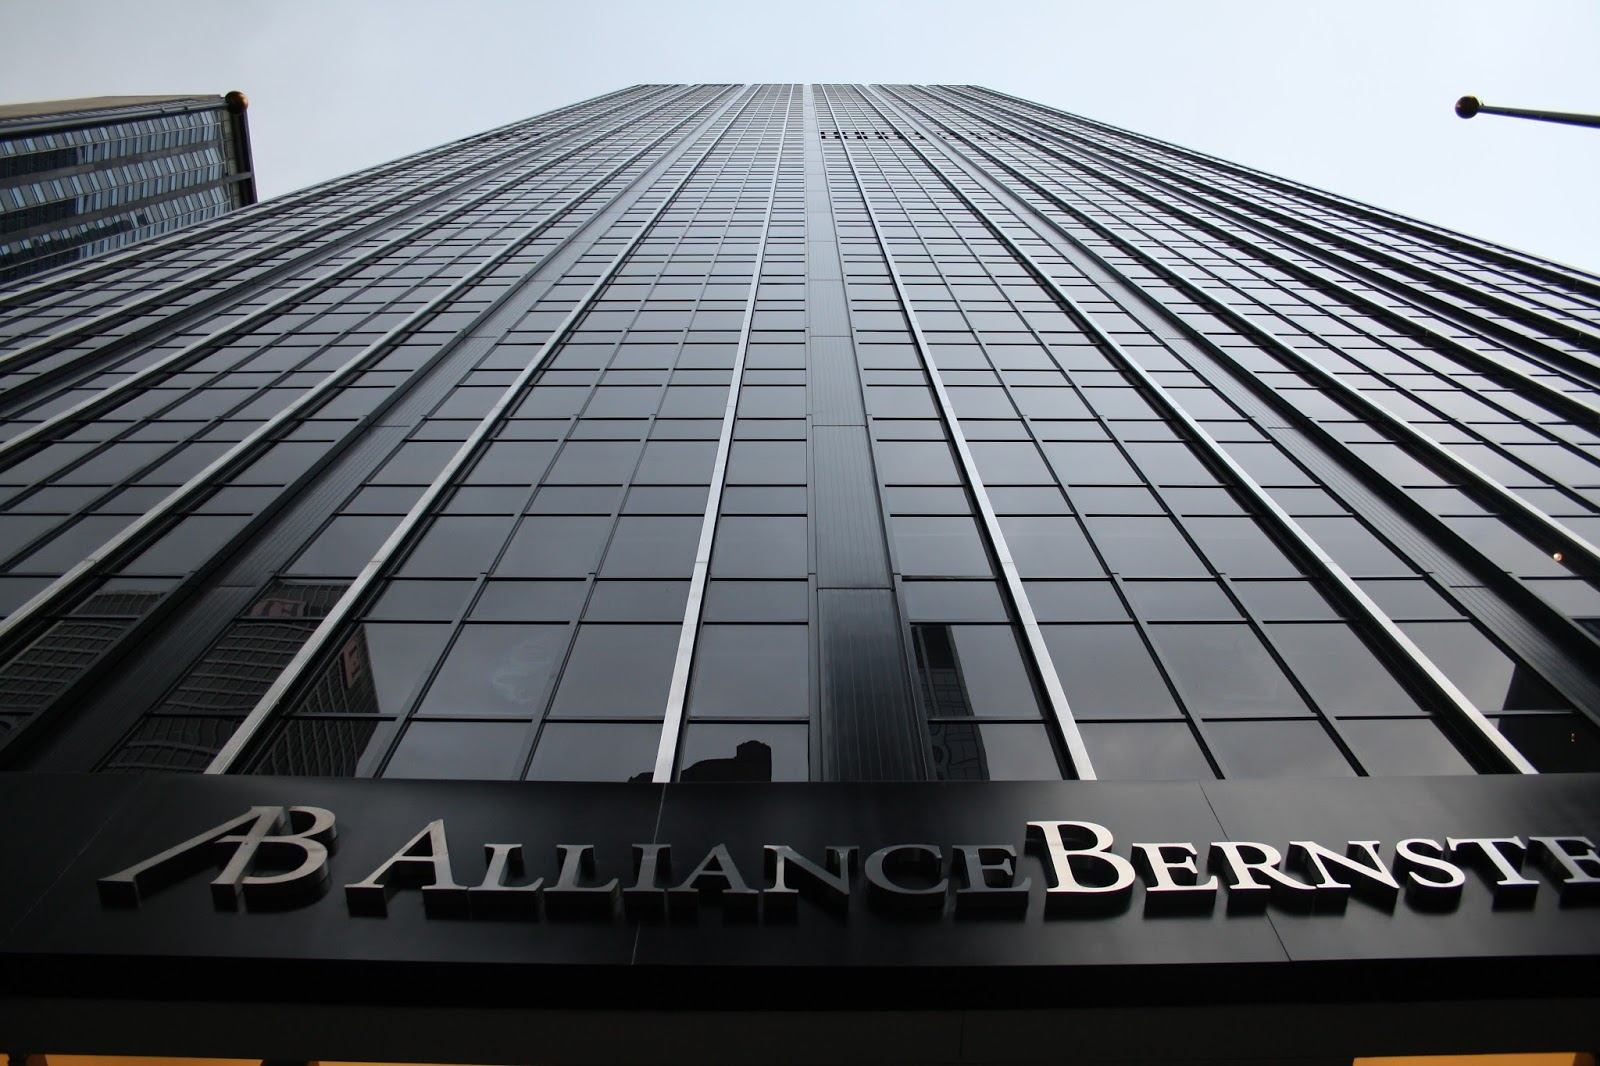
\includegraphics[width=0.45\textwidth]{images/detection-original-image}
      \label{sub:originalimage}
      }
      \\
	\subfloat[Canny - Détection de contours]{
      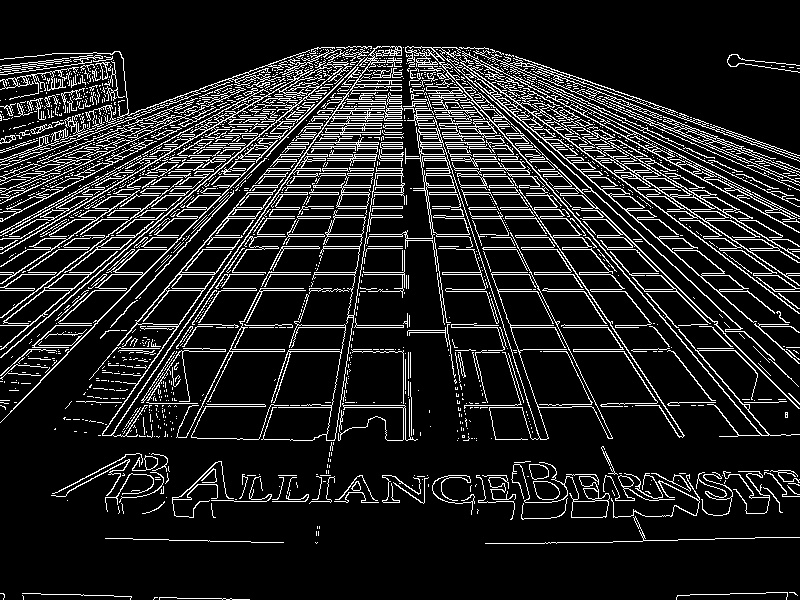
\includegraphics[width=0.45\textwidth]{images/cannysample}
      \label{sub:detectedge}
      }
    \subfloat[Transformée de Hough - Détection de lignes]{
      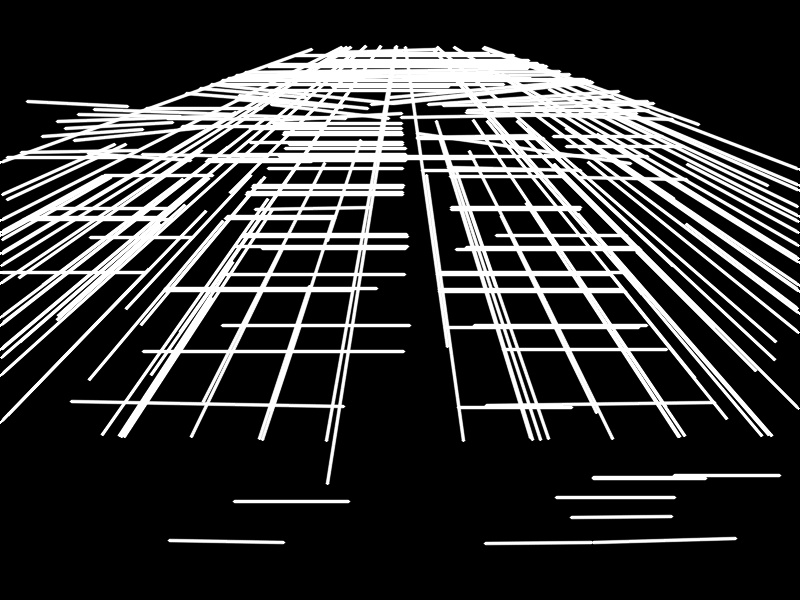
\includegraphics[width=0.45\textwidth]{images/houghsample}
      \label{sub:detectline}
      }
\caption{Détection de lignes : Canny + Hough\protect\footnotemark}
\label{fig:cannyhough}
\end{figure}
\footnotetext{Source : \href{http://funvision.blogspot.com/2016/01/hough-lines-and-canny-edge-sobel.html}{http://funvision.blogspot.com/2016/01/hough-lines-and-canny-edge-sobel.html}}

Cette succession de traitements est cependant lourde et peut difficilement être effectuée en temps réel sur des images haute résolution. 

Dans notre cas, nous nous somme servis de ces deux algorithmes mais uniquement sur des parties d'image (de petite résolution) de façon à améliorer une première détection grossière effectuée notamment à l'aide de marqueurs colorés. Une fois la première détection effectuée, nous obtenons une position plus ou moins précise des quatre coins nécessaires à l'extraction du document. Nous utilisons cette information sur la position potentielle des coins pour extraire des sous-images centrées sur ces coins (fig. ~\ref{sub:subimage:subimage}) que nous seuillons afin d'obtenir une image binaire Figure~\ref{sub:subimage:tresh}. Ensuite, nous appliquons les deux algorithmes mentionnés plus tôt, à savoir la détection de contours (fig. ~\ref{sub:subimage:canny}) puis la détection de lignes (fig. ~\ref{sub:subimage:hough}). Après cela, nous filtrons le résultat de la détection de ligne pour obtenir exactement une ligne verticale et une ligne horizontale. Une fois ces deux lignes trouvées, nous calculons les équations de droite (pente et constante) associées, pour pouvoir en calculer l'intersection et ainsi trouver le coin dans notre sous image (fig ~\ref{sub:subimage:corner}).

\begin{figure}[H]
\centering
	\subfloat[Sous image autour d'un coin.]{
      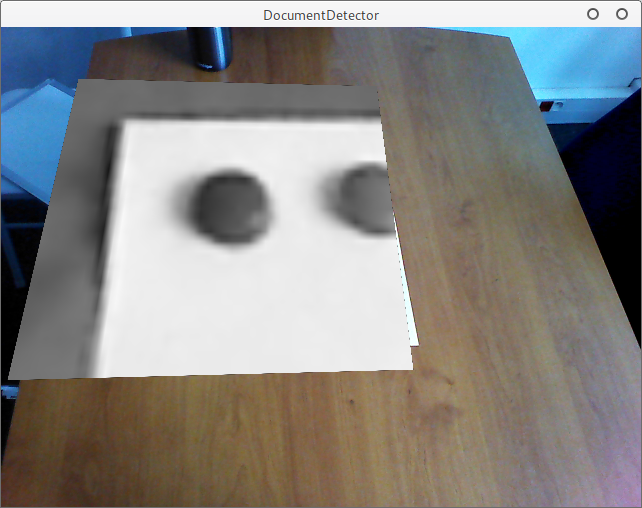
\includegraphics[width=0.33\textwidth]{images/doc-original}
      \label{sub:subimage:subimage}
      }\\
      \subfloat[Seuillage de l'image originale]{
      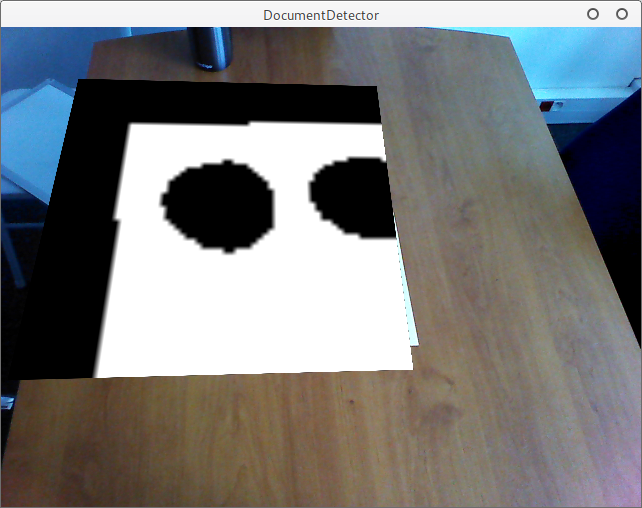
\includegraphics[width=0.33\textwidth]{images/doc-tresh}
      \label{sub:subimage:tresh}
      }
    \subfloat[Canny - Détection de contour basée sur un seuillage de l'image originale]{
      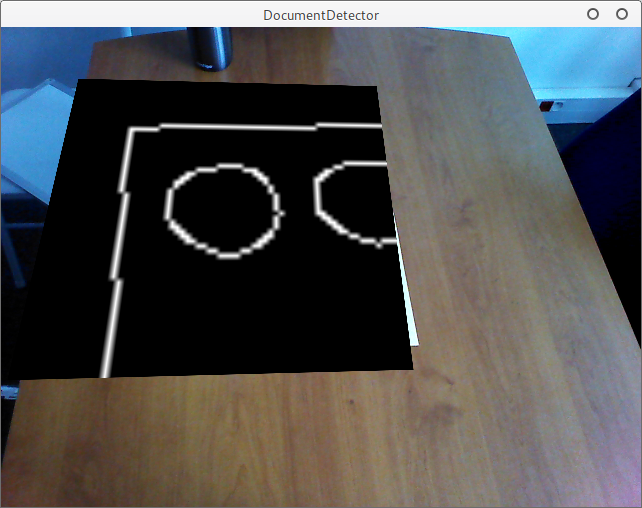
\includegraphics[width=0.33\textwidth]{images/doc-canny}
      \label{sub:subimage:canny}
      }
      \\
	\subfloat[Hough - Détection de lignes basée sur le résultat de Canny]{
      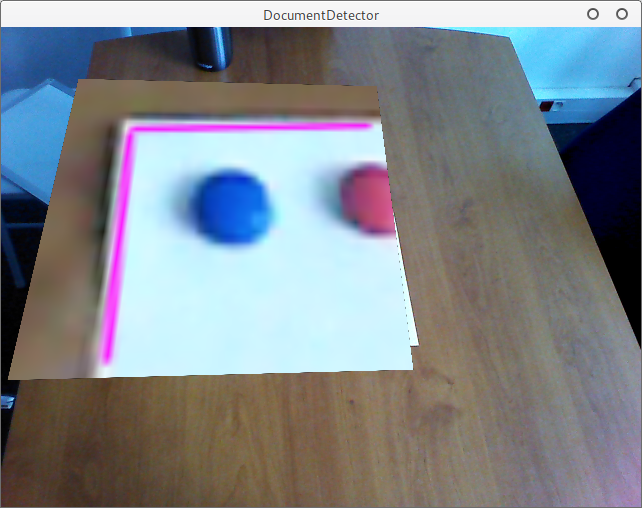
\includegraphics[width=0.33\textwidth]{images/doc-hough}
      \label{sub:subimage:hough}
      }
    \subfloat[Détection finale du coin.]{
      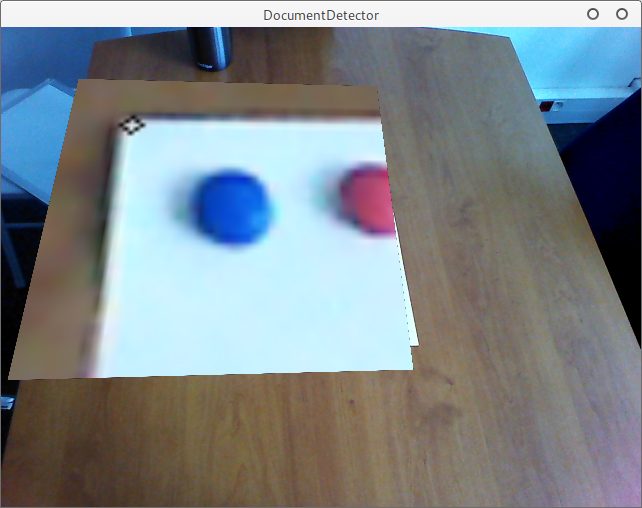
\includegraphics[width=0.33\textwidth]{images/doc-corner}
      \label{sub:subimage:corner}
      }
\caption{Affinage de la détection d'un coin du document}
\label{fig:corner-redetect}
\end{figure}

\subsection{Bilan}
\label{subsec:doc:bilan}
Pour finir, un comparatif des différents résultats obtenus est présenté sur la Figure~\ref{fig:docdetect:results}.
On peut observer quelques points notables : En utilisant Canny puis Hough pour améliorer la détection d'un coin, l'extraction est plus fidèle au document réel Figure~\ref{sub:docdetect:corner} et ~\ref{sub:docdetect:double-corner}. En effet, les coins détectés sont plus précis qu'avec des hypothèses effectuées à priori Figure~\ref{sub:docdetect:simple} et~\ref{sub:docdetect:double}. Toutefois, cette méthode est moins rapide car elle requiert de nombreux calculs supplémentaires. Lorsque utilisée en temps réel, une détection avec connaissance à priori du modèle sera bien plus robuste, car elle ne dépend pas d'une deuxième détection qui à beaucoup de chance d'échouer (seuillage, détection de contours, détection de lignes, intersection entre deux droites puis obtention finale du coin). Ainsi, la méthode à utiliser variera avec les cas d'utilisation. Par exemple, dans le cadre d'une application de scan de document, une méthode d'extraction de document plus précise sera envisagée, mais pour une estimation de pose et un suivi de document il sera préférable d'utiliser une détection plus rapide et robuste.

\begin{figure}[H]
\subfloat[Avec connaissance à priori: Taille du document et distance élément $\longleftrightarrow$ coin]{
      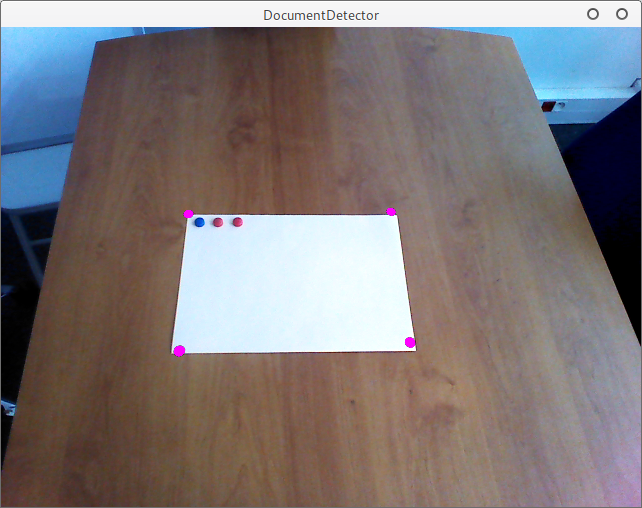
\includegraphics[width=0.5\textwidth]{images/document-detection-simple}
      \label{sub:docdetect:simple}
      }
      \subfloat[Avec connaissance à priori: Taille du document et distance élément $\longleftrightarrow$ coin]{
      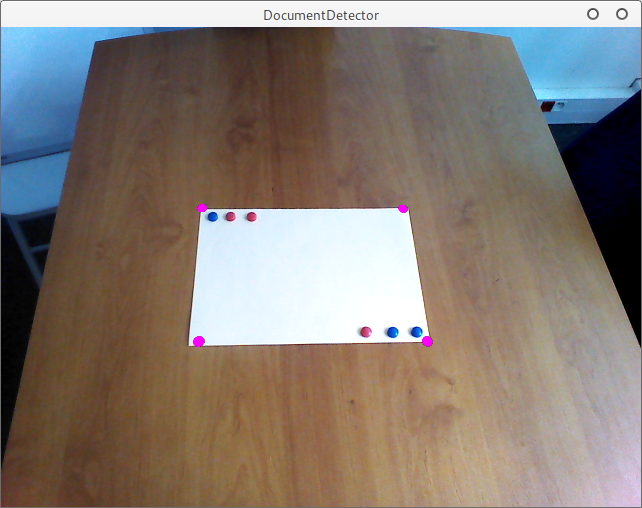
\includegraphics[width=0.5\textwidth]{images/document-detection-double}
      \label{sub:docdetect:double}
      }\\
      \subfloat[Avec connaissance à priori: Taille du document]{
      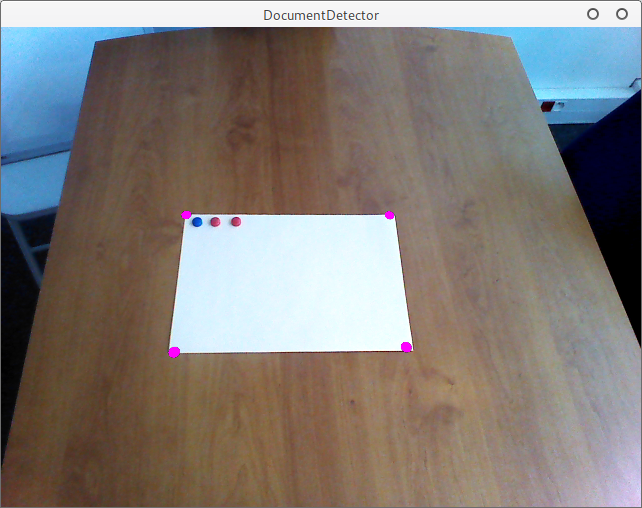
\includegraphics[width=0.5\textwidth]{images/document-detection-corner}
      \label{sub:docdetect:corner}
      }
      \subfloat[Sans connaissance à priori]{
      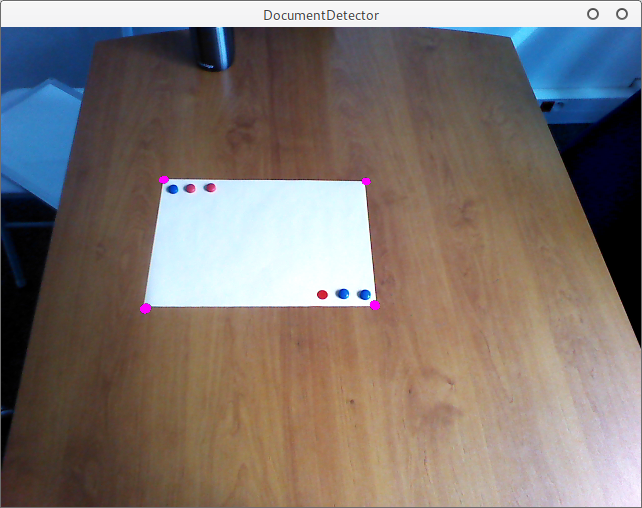
\includegraphics[width=0.5\textwidth]{images/document-detection-double-corner}
      \label{sub:docdetect:double-corner}
      }
      \caption{Résultats des différentes versions de la détection de document.}
      \label{fig:docdetect:results}
\end{figure}


\chapter{Prototype haute performance}
\label{chap:protoHP}

Dans le cadre d'application qu'est la réalité augmentée spatiale, les interactions jouent un rôle majeur dans l'expérience de l'utilisateur. Ainsi, la réactivité, la fluidité de l'expérience et la latence générale du système sont des points cruciaux qu'il est impossible de négliger. Pour pouvoir atteindre ces objectifs et pouvoir pousser les applications encore plus loin, aussi bien dans l'interaction que dans le rendu ou dans le contenu, sans avoir besoin d'une puissance de calcul dépassant l'entendement, une optimisation à la fois logicielle, matérielle et architecturale est nécessaire. 
Cette optimisation a fait l'objet d'une grande partie de mon stage et m'a amené à développer un prototype dit "haute performance" des outils que propose \texttt{RealityTech}. L'optimisation logicielle s'est portée sur l'amélioration des performances des algorithmes de traitement d'image, bien connus pour être extrêmement consommateurs des ressources. Pour l'optimisation matérielle, la tâche fut quelque peu différente. En effet, nous nous sommes attelés à effectuer des mesures et des calculs sur la puissance théorique du matériel, la latence réelle des caméra ainsi que la rapidité de l'encodage des flux vidéos, pour arriver à établir les performances réelles qu'il nous était possible d'atteindre avec différentes combinaisons de matériel. Enfin, le développement du prototype s'est achevé avec la création d'une nouvelle architecture logiciel en micro services\cite{dmitry2014micro}. Le but était de créer un environnement modulaire réactif, où les services peuvent mourir sans pour autant mettre en péril tout le système et ainsi améliorer grandement la qualité générale des outils fournis.

\section{Amélioration logicielle}
\label{sec:hpsoft}
De nos jours, les optimisations font l'objet de développements ciblés et très spécifiques, se concentrant la plupart du temps sur l'amélioration d'un unique point crucial d'un algorithme ou d'une application. Dans notre cas, l'optimisation logicielle a surtout été effectuée au niveau des algorithmes de traitement d'image, omniprésents et indispensables à la technologie. La réalité augmentée spatiale a besoin du monde réel pour exister, c'est pourquoi le matériel se compose de nombreux capteurs (caméras) pour l'analyser et que de nombreux algorithmes de traitement des données captées (images) sont mis en place. 
Après une rapide analyse du logiciel existant, il est indéniable que le traitement le plus utilisé est la convolution d'une image par un filtre qui possède un nombre incalculable d'applications. C'est pourquoi nous avons choisit de concentrer nos efforts sur l'optimisation de ce dernier.

\subsection{Convolution - Théorie}
\label{ssec:convtheo}
\begin{quotation}
\textit{En mathématiques, le produit de convolution est un opérateur bilinéaire et un produit commutatif, généralement noté $∗$, qui, à deux fonctions f et g sur un même domaine infini, fait correspondre une autre fonction $f * g$ sur ce domaine, qui en tout point de celui-ci est égale à l'intégrale sur l'entièreté du domaine (ou la somme si celui-ci est discret) d'une des deux fonctions autour de ce point, pondérée par l'autre fonction autour de l'origine — les deux fonctions étant parcourues en sens contraire l'une de l'autre (nécessaire pour garantir la commutativité).\footnote{Source: \href{https://fr.wikipedia.org/wiki/Produit_de_convolution}{Produit de convolution - Wikipedia}}}
\end{quotation}

Dans le cadre du traitement d'image, le produit de convolution représente une technique de filtrage d'image visant à accentuer ou atténuer certaines caractéristiques de celle-ci telles que la netteté, le flou ou les zones de fort gradient (les contours) par exemple (Figure~\ref{fig:conv:filter}). Étant donné que nous travaillons avec des images définies par un nombre fini de pixels, la convolution d'une image est réalisée dans le domaine discret où $f$ et $g$, dans la définition mathématique, représentent respectivement une image et le filtre qu'on souhaite lui appliquer. Le résultat de cette convolution est une nouvelle image.

On appelle filtre, ou noyau de convolution, une image (ou une matrice), généralement de petite taille, définie en amont, qui va être utilisée pour calculer la nouvelle valeur de chacun des pixels de l'image résultat. C'est la définition de ce dernier qui va décider du traitement appliqué à l'image. 

Le calcul de la valeur d'un pixel dans l'image résultat se fait de la manière suivante : Le voisinage autour du pixel dont on souhaite calculer la valeur est, pondéré par le filtre de convolution que l'on aura préalablement centré sur ce pixel. La nouvelle valeur du pixel représente la somme de toutes les valeurs précédemment calculées (Algorithme~\ref{algo:pseudo:cpu:conv}). Prenons un exemple concret. Sur la Figure~\ref{fig:conv:image}, on souhaite calculer la nouvelle valeur du pixel positionné en 3,3 dans l'image d'origine (I). On sélectionne donc un voisinage de même taille que le filtre (K) centré sur ce pixel, dont chaque élément va être multiplié par la valeur du filtre afin de calculer la valeur du pixel 3,3 dans la nouvelle image soit: 
\begin{center}
$I_{3,3} * K = 88 * 1/9 + 21 * 1/9 + 25 * 1/2 + 68 * 1/9 + 14 * 1/9 + 15 * 1/9 + 35 * 1/9 + 52 * 1/9 + 10 * 1/9 = 36$
\end{center}.

\begin{figure}[H]
\centering
	\subfloat[Image originale]{
      
\includegraphics[width=0.33\textwidth]{images/coffee-identity}
      \label{sub:conv:filter:original}
      }
     \subfloat[Filtre contour]{
      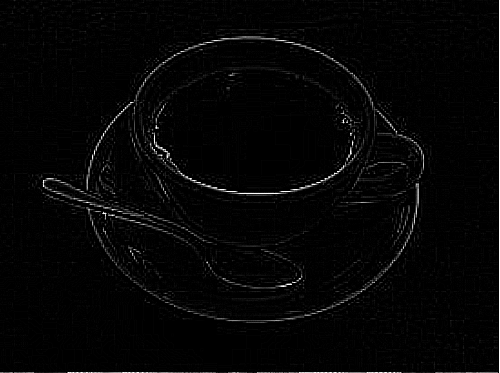
\includegraphics[width=0.33\textwidth]{images/coffee-outline}
      \label{sub:conv:filter:outline}
      }
      \\
      	\subfloat[Filtre de netteté]{
      
\includegraphics[width=0.33\textwidth]{images/coffee-sharpen}
      \label{sub:conv:filter:sharpen}
      }
     \subfloat[Filtre relief]{
      
\includegraphics[width=0.33\textwidth]{images/coffee-emboss}
      \label{sub:conv:filter:emboss}
      }
\caption{Différents filtres de convolution appliqués à une image.}
\label{fig:conv:filter}
\end{figure}

\begin{figure}[H]
\centering
\begin{tikzpicture}
	\matrix (mtr) [matrix of nodes,row sep=-\pgflinewidth, nodes={draw,  minimum size=5.7mm, anchor=center}]
	{
		12 & 46  & 05 & 94 & 25 & 00 & 87\\
		05 & 13  & 01 & 20 & 25 & 00 & 37\\
		72 & 25  & |[fill=red!30]| 88 & |[fill=red!30]| 21 & |[fill=red!30]| 25 & 00 & 99\\
		21 & 74  & |[fill=red!30]| 68 & |[fill=red!30]| 14 & |[fill=red!30]| 15 & 00 & 61\\
		48 & 97  & |[fill=red!30]| 35 & |[fill=red!30]| 52 & |[fill=red!30]| 10 & 00 & 42\\
		11 & 29  & 57 & 00 & 75 & 00 & 12\\
		17 & 01  & 78 & 00 & 50 & 00 & 12\\
		16 & 54  & 00 & 00 & 25 & 00 & 11\\
	};

	\draw[very thick, red] (mtr-3-3.north west) rectangle (mtr-5-5.south east);

	\node [below= of mtr-8-4.south] (lm) {$\bf I$};
	\node[right = 0.2em of mtr] (str) {$* \frac{1}{9}$};

	\matrix (K) [right=0.2em of str,matrix of nodes,row sep=-\pgflinewidth, nodes={draw, fill=blue!30,  minimum size=5.7mm, anchor=center}]
	{
		1 & 1 & 1 \\
		1 & 1 & 1 \\
		1 & 1 & 1 \\
	};
	\node [below = of K-3-2.south] (lk) {$\bf K$};

	\node [right = 0.2em of K] (eq) {$=$};

	\matrix (ret) [right=0.2em of eq,matrix of nodes,row sep=-\pgflinewidth, nodes={draw, minimum size=5.7mm, anchor=center}, nodes in empty cells]
	{
		 &   &  &  &  &  & \\
		 &   &  &  &  &  & \\
		 &   &  &  &  &  & \\
		 &   &  & |[fill=green!30]| 36 &  &  & \\
		 &   &  &  &  &  & \\
		 &   &  &  &  &  & \\
		 &   &  &  &  &  & \\
		 &   &  &  &  &  & \\
	};
	\node [below = of ret-8-4.south] (lim) {${\bf I_{i,j}} * {\bf K}$};

	\draw[very thick, green] (ret-4-4.north west) rectangle (ret-4-4.south east);

	\draw[densely dotted, blue, thick] (mtr-3-3.north west) -- (K-1-1.north west);
	\draw[densely dotted, blue, thick] (mtr-5-3.south west) -- (K-3-1.south west);
	\draw[densely dotted, blue, thick] (mtr-3-5.north east) -- (K-1-3.north east);
	\draw[densely dotted, blue, thick] (mtr-5-5.south east) -- (K-3-3.south east);

	\draw[densely dotted, green, thick] (ret-4-4.north west) -- (K-1-1.north west);
	\draw[densely dotted, green, thick] (ret-4-4.south west) -- (K-3-1.south west);
	\draw[densely dotted, green, thick] (ret-4-4.north east) -- (K-1-3.north east);
	\draw[densely dotted, green, thick] (ret-4-4.south east) -- (K-3-3.south east);

	\draw[very thick, blue] (K-1-1.north west) rectangle (K-3-3.south east);

	\node[anchor=south east, inner sep=0.01em, blue] at (mtr-3-3.south east) (xx) {\scalebox{.5}{$\times 1$}};
	\node[anchor=south east, inner sep=0.01em, blue] at (mtr-3-4.south east) (xx) {\scalebox{.5}{$\times 1$}};
	\node[anchor=south east, inner sep=0.01em, blue] at (mtr-3-5.south east) (xx) {\scalebox{.5}{$\times 1$}};
	\node[anchor=south east, inner sep=0.01em, blue] at (mtr-4-3.south east) (xx) {\scalebox{.5}{$\times 1$}};
	\node[anchor=south east, inner sep=0.01em, blue] at (mtr-4-4.south east) (xx) {\scalebox{.5}{$\times 1$}};
	\node[anchor=south east, inner sep=0.01em, blue] at (mtr-4-5.south east) (xx) {\scalebox{.5}{$\times 1$}};
	\node[anchor=south east, inner sep=0.01em, blue] at (mtr-5-3.south east) (xx) {\scalebox{.5}{$\times 1$}};
	\node[anchor=south east, inner sep=0.01em, blue] at (mtr-5-4.south east) (xx) {\scalebox{.5}{$\times 1$}};
	\node[anchor=south east, inner sep=0.01em, blue] at (mtr-5-5.south east) (xx) {\scalebox{.5}{$\times 1$}};
\end{tikzpicture}
\caption{Convolution d'une matrice (image) (I) par un filtre (K)}
\label{fig:conv:image}
\end{figure}

\begin{algorithm}[H]
	\caption{Convolution d'une image par un filtre}
	\begin{algorithmic}
		\Procedure{Convolution}{I, K, Iw, Ih, Ks}\Comment{I: image, K: filtre}
		\State $I_{conv} \gets I$
		\State $Khs \gets floor(Ks \div 2)$
		\State $x \gets 0, y \gets 0$
		\State $sum \gets 0$
		\For{$x \leq Iw ; ++x$}
			\For{$y \leq Ih ; ++y$}\Comment{Pour tous les pixels $x,y$}
			\State $maskSum \gets 0$
				\For{$i \leq Ks ; ++j$}
					\For{$j \leq Ks ; ++j$}\Comment{Pour chaque élément dans une fenêtre de taille $Ks$}
					\State ${pos_x \gets x + i - Khs}$ \Comment{pos = pos + position dans le voisinage}
					\State ${pos_y \gets y + j - Khs}$ \Comment{pos = pos + position dans le voisinage}
					\If{$outOf(I, pos_x, pos_y)$} \Comment{Vérifie que les positions sont dans l'image (bords)}
						\State $continue$
					\EndIf
					\State $sum \gets sum + I_{pos_x, pos_y} * K{i, j}$ \Comment{Somme du voisinage par le filtre}
					\State $maskSum \gets maskSum + K{i, j}$
					\EndFor
				\EndFor
				\State $I_{conv}{x, y} \gets sum \div maskSum$ \Comment{Valeur finale = somme normalisée}
			\EndFor
		\EndFor
		\State \Return $I_{conv}$ \Comment{Retourne la nouvelle image}
		\EndProcedure
	\end{algorithmic}
	\label{algo:pseudo:cpu:conv}
\end{algorithm}

Comme on peut s'en rendre compte dans le pseudo code proposé ci-dessus (Algorithme~\ref{algo:pseudo:cpu:conv}), l'image résultat est une nouvelle image (indépendante de l'image d'origine) dont chaque pixel a été calculé indépendamment de ces voisins dans cette nouvelle image. Cela signifie que n'importe quel pixel peut être calculé dans n'importe quel ordre. C'est précisément à cette propriété que nous allons nous intéresser car, en théorie, avec une puissance de calcul suffisante il est possible de calculer en même temps tous les pixels de l'image résultat. Cet algorithme possède donc un très fort potentiel d'optimisation car il est très largement parallélisable.

\subsection{Convolution - Optimisation}
L'optimisation de cet algorithme peut se faire de deux façons bien distinctes. La première se fait en utilisant la puissance de la carte graphique de l'ordinateur pour effectuer énormément de calculs en même temps. C'est l'optimisation sur carte graphique dont nous avons évoqué le principe dans le Chapitre~\ref{chap:notions}. La seconde méthode d'optimisation consiste à légèrement changer l'algorithme de convolution: la convolution est séparée en deux filtres distincts\cite{podlozhnyuk2007image}, un horizontal et un vertical, qui sont successivement appliqués à l'image origine (Figure~\ref{fig:conv:separable}). Ainsi, la complexité d'appliquer une convolution de taille $MxM$ à une image de taille $NxN$ est réduit de $O(N^2M^2)$ à $O(N^2M)$ puisqu'au lieu de parcourir pour chaque pixel un voisinage de taille $MxM = M ^2$ il suffit de parcourir $2xM$ pixels soit $M$.

\begin{figure}[H]
\centering
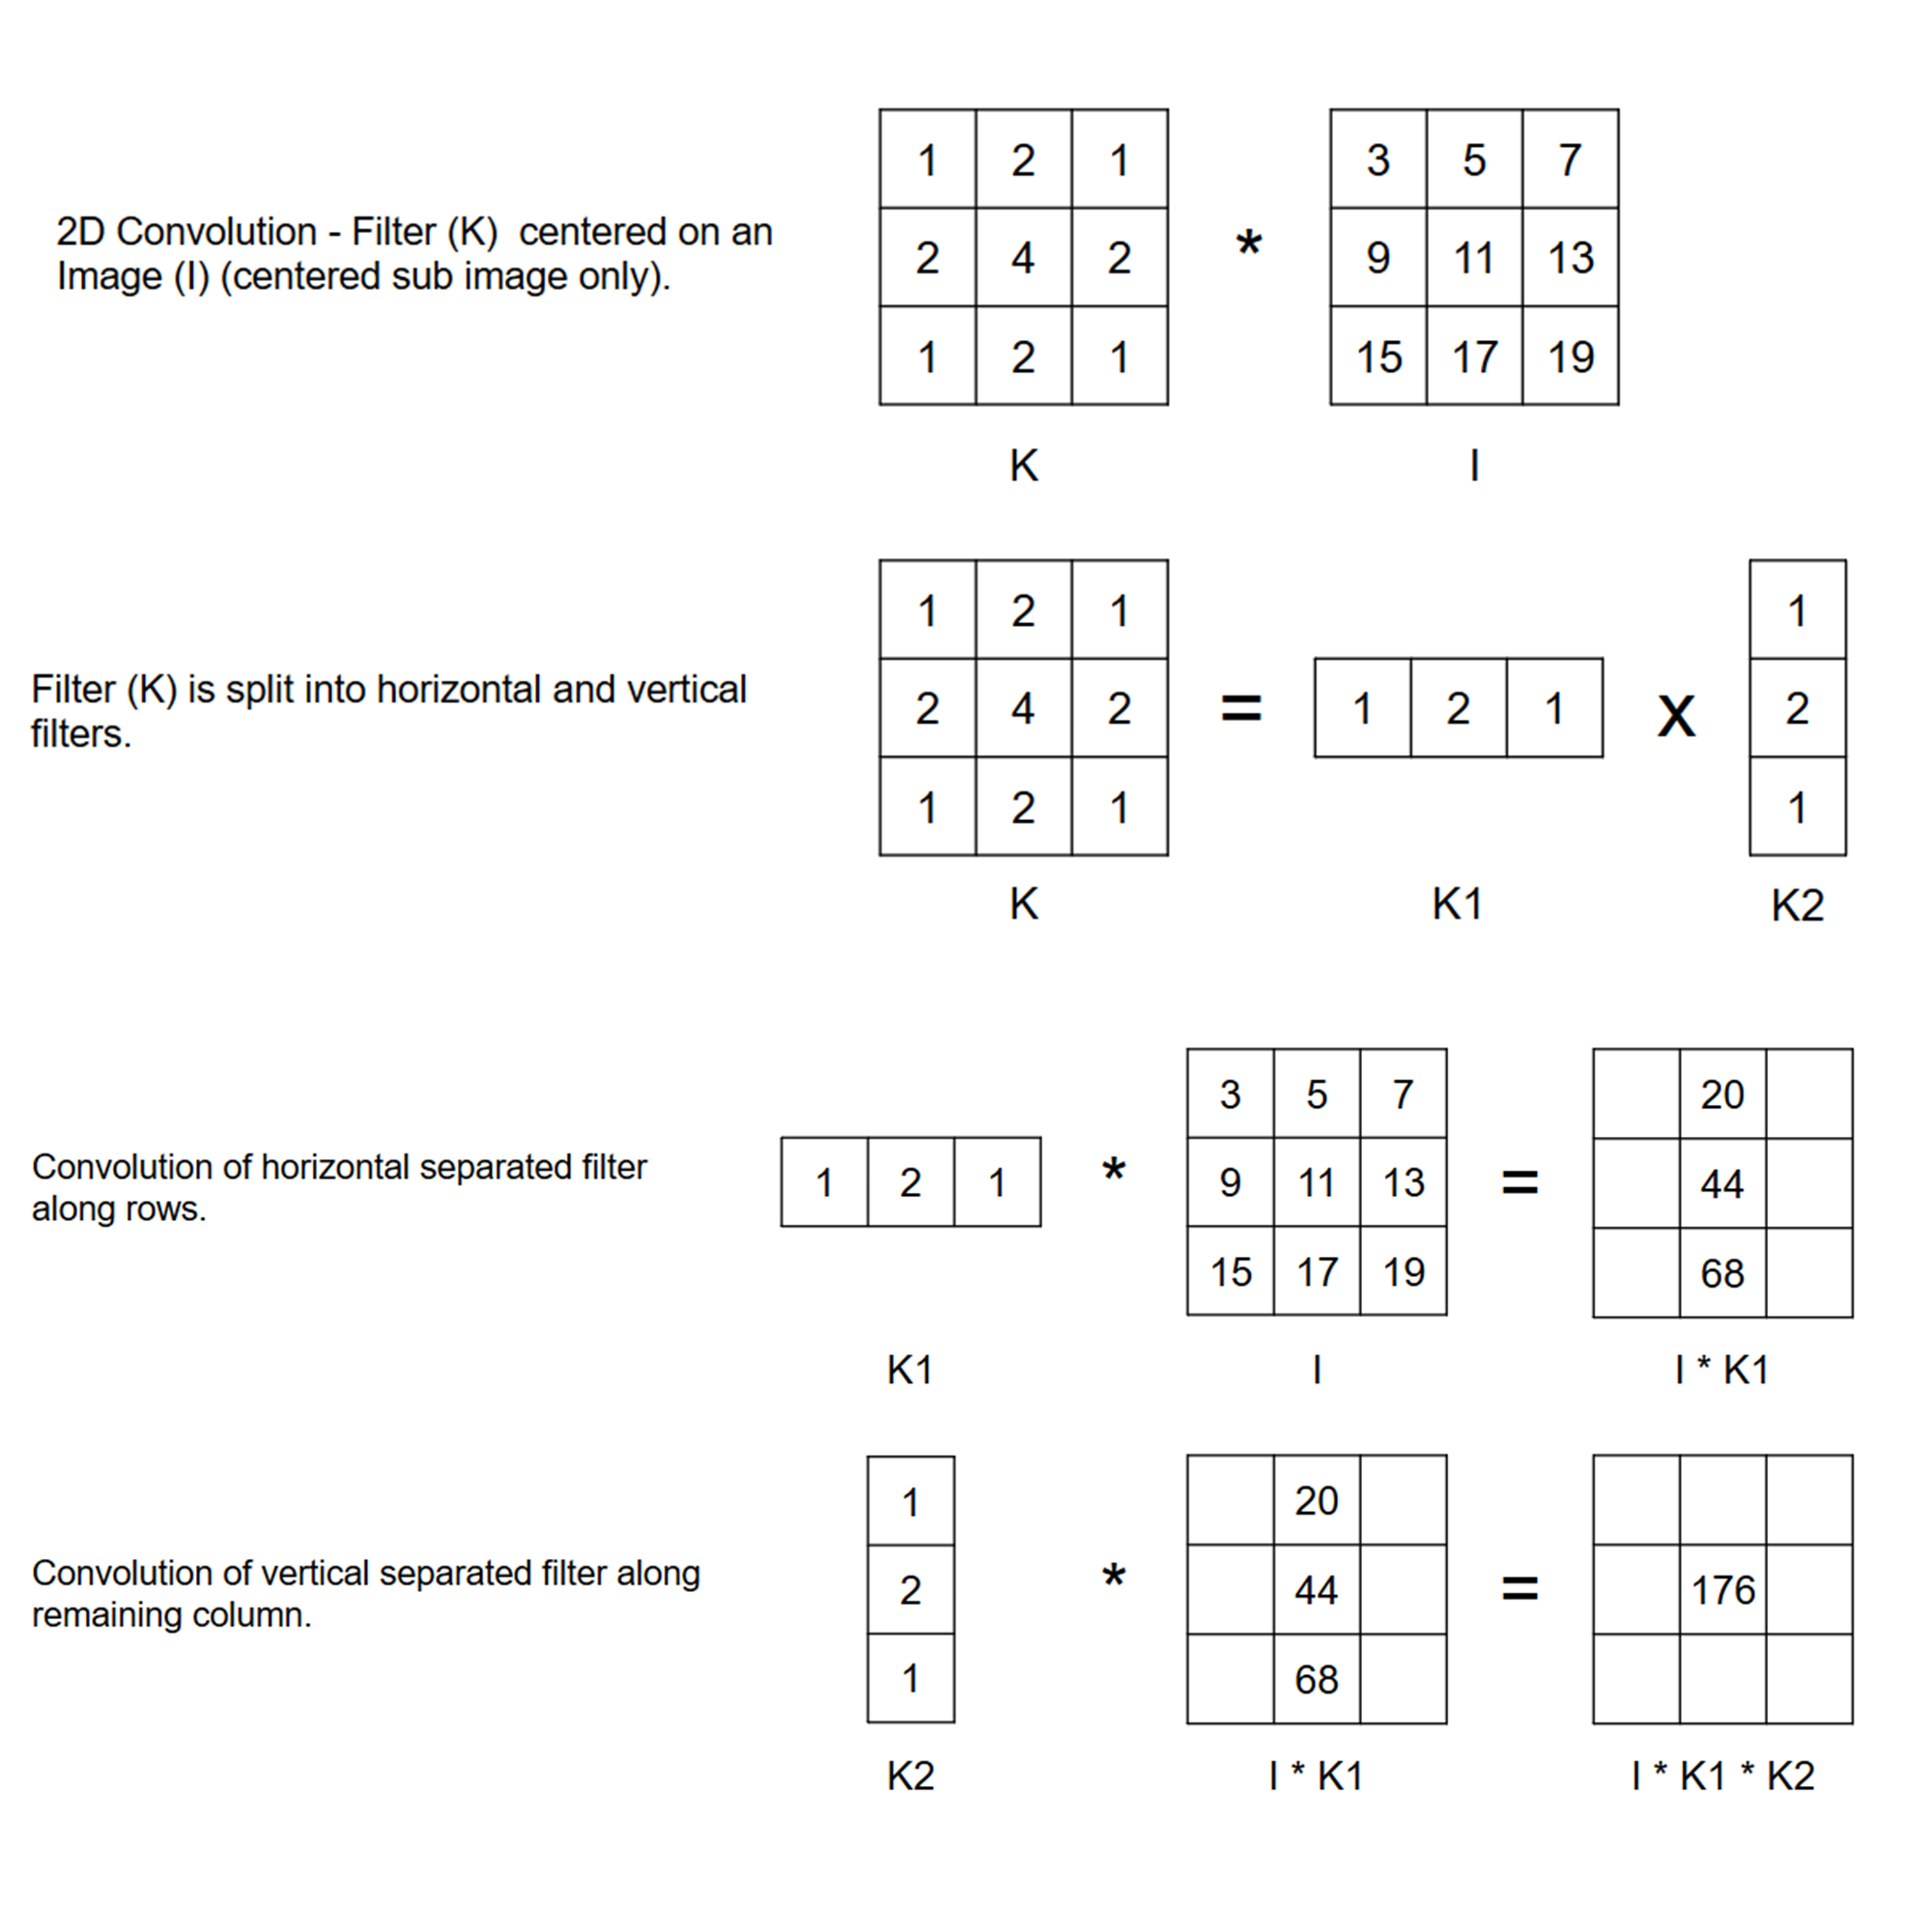
\includegraphics[width=0.7\linewidth]{images/separableconv}
\caption{Exemple d'un filtre de convolution appliqué successivement horizontalement puis verticalement}
\label{fig:conv:separable}
\end{figure}

Nous avons choisi de n'effectuer que l'optimisation sur carte graphique car la deuxième méthode comporte un gros coût en complexité et temps de développement que nous n'avons pas jugé nécessaire d'inclure dans cette première version. De plus, il n'est pas toujours possible de séparer un filtre $K$ en deux sous-filtres $K1, K2$ tel que $K = K1 \times K2$.

Pour pouvoir développer ladite optimisation, il a fallut utiliser un langage de programmation sur carte graphique. De nos jours, il en existe plusieurs et ils possèdent tous leurs spécificités. Cependant, pendant la phase de recherche, trois langages (ou sous-langages) se sont démarqués : OpenCL\cite{opencl}, OpenGL ES\cite{opengles} et CUDA\cite{cuda}. Nous avons donc choisi d'implémenter trois versions de l'algorithme de convolution naïf (non séparé) utilisant chacun de ces langages, afin d'en évaluer et comparer les performances.

\subsection{OpenCL} 
OpenCL ou \emph{Open Computing Language} est un langage de programmation basé sur le C, créé par \texttt{Khronos Group} en 2009.
Un programme OpenCL s'écrit en deux parties : La partie \textbf{code hôte} et la partie \textbf{noyau} ou \textbf{code périphérique}, qui représentent respectivement la partie application se chargeant d'orchestrer les différentes tâches, la gestion mémoire ainsi que la gestion des périphériques s'exécutant sur l'hôte et la partie calcul permettant de compléter lesdites tâches s'exécutant sur les périphériques. La partie hôte est écrite en C tandis que la partie noyau est écrite en OpenCL-C.
Il faut donc bien différencier hôte et périphérique (Figure~\ref{fig:opencl}). Dans notre cas d'utilisation, l'hôte représente le processeur et permet de transmettre les données aux périphériques qui, ici, correspondent à une ou plusieurs cartes graphiques.

\begin{figure}[H]
\centering
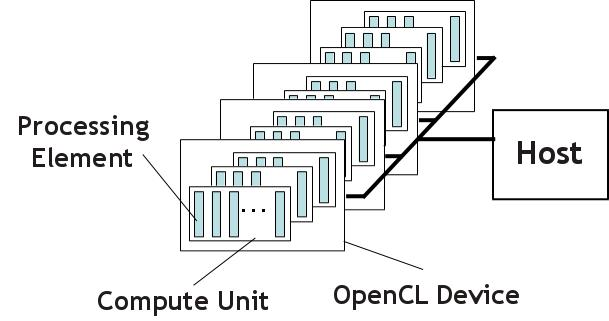
\includegraphics[width=0.5\linewidth]{images/opencl}
\caption{Schéma OpenCL - Hôte et périphériques\protect\footnotemark}
\label{fig:opencl}
\end{figure}

\footnotetext{Source: \href{https://www.anandtech.com/show/7334/a-look-at-alteras-opencl-sdk-for-fpgas/2}{https://www.anandtech.com/show/7334/a-look-at-alteras-opencl-sdk-for-fpgas/2}}

Nous nous sommes intéressés à OpenCL car il est compatible avec la plupart des systèmes et des architectures aujourd'hui présents sur le marché, sans aucune modification de code nécessaire. Cet avantage est aussi l'un de ses plus gros inconvénients puisqu'il ne permet pas d'exploiter au mieux chaque architecture comme peut le faire CUDA avec NVIDIA, et les performances de ce dernier ne sont donc pas équivalentes sur chaque architecture. %Parler dans le bilan Le coût de développement de traitement en OpenCL tout aussi lourd

\subsection{OpenGL (ES)}
OpenGL est une interface de programmation multi-plateforme et multi-langage permettant de faire le rendu de scènes 3D. En tant qu'interface, il est possible de l'implémenter de façon logicielle mais elle a été conçue pour être implémentée de manière matérielle afin de profiter au mieux des accélérations dédiées disponibles. Ainsi, c'est grâce à ces implémentations qu'OpenGL fournit un \emph{pipeline} programmable de rendu ultra performant. C'est justement par le biais de ce dernier programmable et plus spécifiquement via le code hôte et les shaders qu'il est possible de transmettre des instructions et des données à la carte graphique (Figure~\ref{fig:opengl:pipeline})

\begin{figure}[H]
\centering
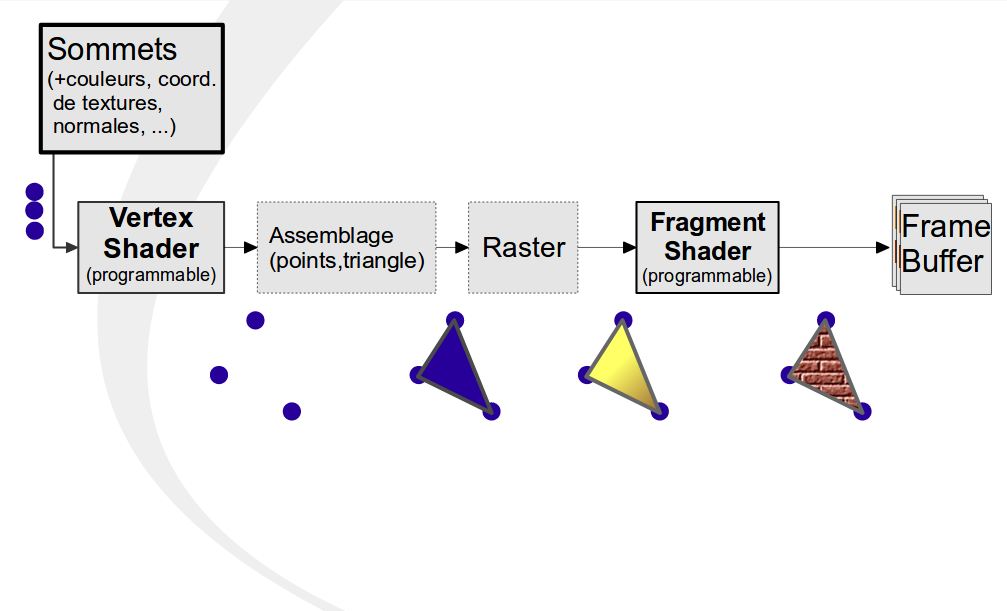
\includegraphics[width=0.7\linewidth]{images/opengl-pipeline}
\caption{Pipeline de rendu - OpenGL\protect\footnotemark}
\label{fig:opengl:pipeline}
\end{figure}

\footnotetext{Source: \href{http://www.labri.fr/perso/pbenard/teaching/mondes3d/slides/Cours_Monde3D_2017_04-IntroGL.pdf}{Cours M1 Informatique - Mondes 3D - Pierre Benard}}

Le pipeline OpenGL reçoit en entrée:
\begin{itemize}
\item Des informations sur la géométrie de la scène.
\item Des paramètres nécessaires pour effectuer le rendu de la scène (point de vue de la caméra, lumières, textures, matériaux).
\end{itemize}
et donne en sortie une image de la scène.

Pour pouvoir utiliser ce pipeline dans l'optique d'opérer des traitements sur des images 2D, il est nécessaire d'en détourner l'utilisation. En effet, sans géométrie à fournir au vertex shader, le pipeline de rendu ne se déclenche pas. L'idée, pour passer outre, est de créer un bout de géométrie recouvrant l'écran (le plus souvent un quad) afin d'activer le pipeline de rendu. Une fois activé, le vertex shader est programmé pour ne rien faire. Les étapes d'assemblage et de rastérisation sont, de ce fait, très rapidement achevées et l'étape du rendu par fragment peut alors débuter. L'image de sortie du rendu est composée dans le fragment shader, c'est donc ici que nous avons accès à chacun des pixels composant l'image finale. Le code présent dans ce shader permet d'effectuer, pour chaque pixel, le calcul de la convolution. Une fois le traitement par fragment effectué, l'image résultat est stockée dans le \emph{Frame Buffer Object ou FBO} et peut être récupérée depuis l'hôte.

L'avantage de cette technique est que, comme OpenCL, OpenGL (ES) est largement compatible avec toutes les plateformes et est très largement utilisé. Cependant, contrairement à OpenCL, les performances d'OpenGL ne dépendent que du matériel, ainsi, elles ne varieront pas, ou très peu, d'une architecture à un autre. Ainsi pour une puissance de calcul théorique identique et mais une architecture différente les performances seront quasiment équivalentes.

\subsection{CUDA} 
A la différence d'OpenCL et d'OpenGL, CUDA n'est pas seulement un langage de programmation mais bel et bien une architecture de traitement parallèle développée par NVIDIA. Son unique but est d'exploiter la carte graphique à son maximum, pour offrir une énorme puissance de calcul au système l'utilisant. Pour ce qui est de la partie programmation, NVIDIA fournit une API permettant d'utiliser cette architecture, CUDA C, et qui fonctionne de façon similaire à OpenCL avec du code hôte et du code périphérique qui seront les noyaux CUDA à exécuter sur la carte graphique. Là où CUDA se démarque c'est dans le modèle qu'il propose : les tâches (\emph{threads}) sont regroupées en blocs (\emph{blocks}) à l'intérieur desquels la mémoire est partagée. De plus, chaque bloc s'exécute sur exactement une unité de calcul (Figure~\ref{fig:cuda:archi}). Par ailleurs, la mémoire est unifiée (Figure~\ref{fig:cuda:unifiedmemory}), de ce fait, les CPUs et les GPUs travaillant ensemble ont accès à la même mémoire, ce qui permet d'éviter bon nombre de copies et ainsi réduire considérablement les temps de transfert de données.

\begin{figure}[H]
\centering
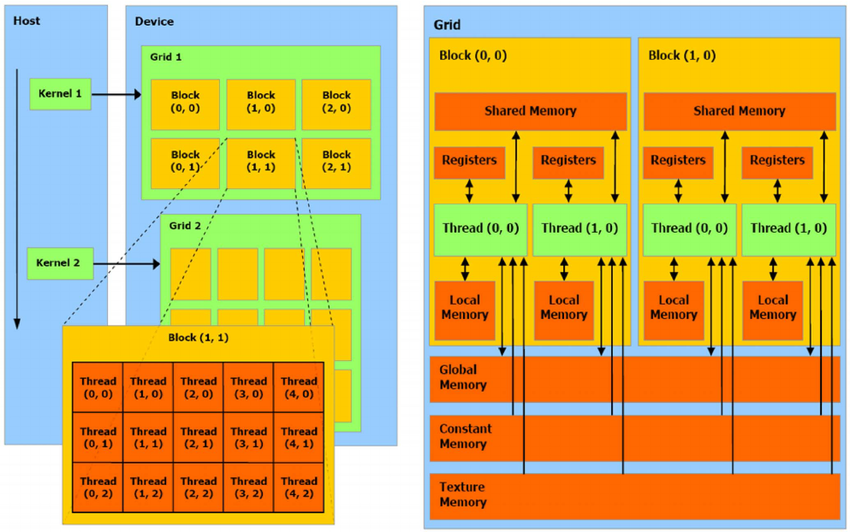
\includegraphics[width=0.9\linewidth]{images/cuda-archi}
\caption{Représentation schématique de l'architecture CUDA\protect\footnotemark}
\label{fig:cuda:archi}
\end{figure}
\footnotetext{Source: \href{http://programming4.us/enterprise/18672.aspx}{NVIDIA CUDA - Unified Device Architecture}}

\begin{figure}[H]
\centering
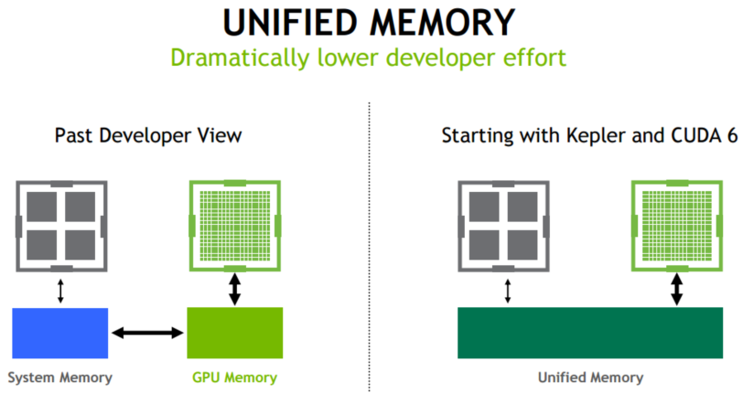
\includegraphics[width=0.65\linewidth]{images/cuda-unified-memory}
\caption{Mémoire séparée vs mémoire unifiée\protect\footnotemark}
\label{fig:cuda:unifiedmemory}
\end{figure}
\footnotetext{Source: \href{https://devblogs.nvidia.com/unified-memory-cuda-beginners/}{NVIDIA CUDA - Unified Memory for beginners}}

CUDA étant une architecture matérielle, seules les cartes graphiques NVIDIA récentes en sont équipées, ce qui, contrairement aux deux autres, ne la rend absolument pas multi-plateforme.

\subsection{Tests de performance}
\label{sub:conv:bench}
Afin de comparer les différentes solutions, nous avons réalisé des tests de performance du même algorithme de convolution, que nous avons implémenté dans les différents langages cités et sur différentes machines avec des configurations bien différentes. Le but de ces tests était, dans un premier temps, d'observer l'impact de l'optimisation et dans un second temps, d'orienter le choix d'ordinateur à inclure dans le système de RealityTech en se basant sur les résultats obtenus en fonction des différentes plateformes.

\textbf{Note:} L'algorithme de convolution implémenté est la version non séparé où le filtre de convolution est considéré comme une matrice.

\textbf{Note 2:} Nous avons choisit de ne pas réalisé les tests de performance OpenCL car nous avons jugé que cette technologie comportait beaucoup de trop de défauts et n'était donc pas pertinente.

Dans ce test de performance, nous avons mesuré plusieurs choses :
\begin{itemize}
\item \textbf{Le temps de transfert} des données de l'hôte au périphérique. Cette mesure est importante car elle permet d'évaluer le coût des opération de transfert et de ce fait l'impact de la mémoire unifiée CUDA par rapport aux autres méthodes ne possédant pas cette fonctionnalité.
\item \textbf{Le temps de calcul} brut de la convolution de l'image. Afin d'évaluer les performances brutes de l'algorithme par langage, nous avons mesuré le temps nécessaire au filtrage d'une image avec un noyau donné. Le temps de calcul ne prends donc en compte que le strict minimum des opérations nécessaires au calcul. Les allocations de variable, de mémoire etc. ne sont donc pas prises en compte dans ce temps.
\item \textbf{La "bande passante"} du traitement entier, comprenant transfert calcul et re transfert. Cette mesure donne une bonne idée de la rapidité des algorithmes car elle exprime le nombre de méga octet qu'il est possible de traiter en une seconde avec chaque implémentation.
\end{itemize}

\textbf{Note:} Les résultats présentés dans les tableaux~\ref{fig:bench:cuda},~\ref{fig:bench:opengles},~\ref{fig:bench:cpu} ont été mesurés sur le kit de développement NVIDIA Tegra Jetson TX2 dont les spécificités sont les suivantes: \texttt{CPU ARM ARM Cortex-A57 (quad-core) @ 2GHz + NVIDIA Denver2 (dual-core) @ 2GHz, GPU 256-core Pascal @ 1300MHz, RAM 8GB 128-bit LPDDR4 @ 1866Mhz |  59.7 GB/s}. Nous avons choisi d'exposer ici seulement les résultats obtenus sur le kit de developpement NVIDIA car il permet d'observer les performances de CUDA dans un environnement ultra optimisé pour ce dernier cependant vous trouverez en Annexe 1 les résultats de ces mêmes tests effectués sur plusieurs ordinateurs différents.

\begin{table}[H]
\centering
\caption{CUDA 9.0 - Convolution d'une image en niveau de gris par un filtre de taille 5x5 - float 32bits}
\label{fig:bench:cuda}
\resizebox{\textwidth}{!}{%
\begin{tabular}{|c|c|c|c|c|c|}
\hline
\textbf{Size} & \textbf{Size (MB)} & \textbf{Compute Time (ms)} & \textbf{Transfer Time (ms)} & \textbf{Total Time (ms)} & \textbf{Bandwidth (MB/s)} \\ \hline
\cellcolor{green!40}\textbf{128x128} & 0,0655 & 0,0964 & 0,7737 & \cellcolor{green!40}0,8701 & 75,3224 \\ \hline
\cellcolor{green!40}\textbf{256x256} & 0,2621 & 0,2222 & 1,8457 & \cellcolor{green!40}2,0679 & 126,7661 \\ \hline
\cellcolor{green!40}\textbf{512x512} & 1,0486 & 0,8764 & 3,5266 & \cellcolor{green!40}4,4030 & 238,1503 \\ \hline
\cellcolor{green!40}\textbf{1024x1024} & 4,1943 & 3,2107 & 9,1959 & \cellcolor{green!40}12,4066 & 338,0703 \\ \hline
\cellcolor{orange!70}\textbf{2048x2048} & 16,7772 & 12,7048 & 35,0284 & \cellcolor{orange!70}47,7332 & 351,4786 \\ \hline
\cellcolor{red!40}\textbf{4096x4096} & 67,1089 & 51,0330 & 139,0710 & \cellcolor{red!40}190,1040 & 353,0115 \\ \hline
\cellcolor{red!40}\textbf{8192x8192} & 268,4350 & 210,2130 & 553,8050 & \cellcolor{red!40}764,0180 & 351,3464 \\ \hline
\end{tabular}%
}
\end{table}

\begin{table}[H]
\centering
\caption{OpenGL ES 2.0 - Convolution d'une image en niveau de gris par un filtre de taille 5x5 - float 32bits}
\label{fig:bench:opengles}
\resizebox{\textwidth}{!}{%
\begin{tabular}{|c|c|c|c|c|c|}
\hline
\textbf{Size} & \textbf{Size (MB)} & \textbf{Compute Time (ms)} & \textbf{Transfer Time (ms)} & \textbf{Total Time (ms)} & \textbf{Bandwidth (MB/s)} \\ \hline
\cellcolor{green!40}\textbf{128x128} & 0,0655 & 0,1386 & 0,9038 & \cellcolor{green!40}1,0424 & 62,8703 \\ \hline
\cellcolor{green!40}\textbf{256x256} & 0,2621 & 0,0202 & 1,3858 & \cellcolor{green!40}1,4060 & 186,4475 \\ \hline
\cellcolor{green!40}\textbf{512x512} & 1,0486 & 0,0194 & 4,2613 & \cellcolor{green!40}4,2807 & 244,9576 \\ \hline
\cellcolor{green!40}\textbf{1024x1024} & 4,1943 & 0,0212 & 15,6039 & \cellcolor{green!40}15,6251 & 268,4337 \\ \hline
\cellcolor{red!40}\textbf{2048x2048} & 16,7772 & 0,0215 & 60,8093 & \cellcolor{red!40}60,8309 & 275,8008 \\ \hline
\cellcolor{red!40}\textbf{4096x4096} & 67,1089 & 0,0215 & 241,5410 & \cellcolor{red!40}241,5625 & 277,8117 \\ \hline
\cellcolor{red!40}\textbf{8192x8192} & 268,4350 & 0,0267 & 1163,1867 & \cellcolor{red!40}1163,2133 & 230,7702 \\ \hline
\end{tabular}%
}
\end{table}

\begin{table}[H]
\centering
\caption{CPU - Convolution d'une image en niveau de gris par un filtre de taille 5x5 - float 32bits}
\label{fig:bench:cpu}
\resizebox{\textwidth}{!}{%
\begin{tabular}{|c|c|c|c|c|c|}
\hline
\textbf{Size} & \textbf{Size (MB)} & \textbf{Compute Time (ms)} & \textbf{Transfer Time (ms)} & \textbf{Total Time (ms)} & \textbf{Bandwidth (MB/s)} \\ \hline
\cellcolor{green!40}\textbf{128x128} & 0,0655 & 8,3513 & 0,0000 & \cellcolor{green!40}8,3569 & 7,8421 \\ \hline
\cellcolor{green!40}\textbf{256x256} & 0,2621 & 33,8604 & 0,0000 & \cellcolor{green!40}33,8698 & 7,7398 \\ \hline
\cellcolor{red!40}\textbf{512x512} & 1,0486 & 150,1860 & 0,0000 & \cellcolor{red!40}150,2010 & 6,9812 \\ \hline
\cellcolor{red!40}\textbf{1024x1024} & 4,1943 & 721,2130 & 0,0000 & \cellcolor{red!40}721,2310 & 5,8155 \\ \hline
\cellcolor{red!40}\textbf{2048x2048} & 16,7772 & 3196,6300 & 0,0000 & \cellcolor{red!40}3196,6500 & 5,2484 \\ \hline
\cellcolor{red!40}\textbf{4096x4096} & 67,1089 & 13130,9000 & 0,0000 & \cellcolor{red!40}13130,9000 & 5,1108 \\ \hline
\cellcolor{red!40}\textbf{8192x8192} & 268,4350 & 53591,6000 & 0,0000 & \cellcolor{red!40}53591,7000 & 5,0089 \\ \hline
\end{tabular}%
}
\end{table}

Comme on peut s'en rendre compte, les gains de performance des deux versions optimisées de l'algorithme sont non négligeables par rapport à la version CPU naïve (Figure~\ref{fig:bench:cpu}). En effet, on observe que les algorithmes s'exécutant sur la carte graphique sont jusqu'à 55 fois plus rapide pour OpenGL ES (Figure~\ref{fig:bench:opengles}) et jusqu'à 70 fois pour la version CUDA (Figure~\ref{fig:bench:cuda}). Les cases vertes dans les tableaux indiquent que l'image a pu être traitée en pseudo temps réel avec une fréquence de rafraichissement de 25 images par seconde (IPS) ou \emph{Frames Per Second (FPS)}, ce qui signifie que pour chaque image à afficher, nous disposons d'un temps de $1/25 * 1000 = 40$ millisecondes pour en faire le rendu. Au delà de ce constat d'optimisation, on peut voir que la version CUDA et la version OpenGL affichent des résultats plutôt similaires puisqu'ils sont tout deux capables de traiter en temps réel des images de taille 1024x1024 pixels sans difficulté. Toutefois, on note quand même une différence flagrante entre ces deux versions. En effet, on peut observer le gain apporté par la mémoire unifiée CUDA lorsque l'on compare les temps de transfert avec ceux d'OpenGL. En moyenne les temps de transfert en CUDA (pour des images haute résolution) sont environ deux fois plus rapide que leurs équivalents OpenGL ES, ce qui a un impact significatif sur les performances car ils correspondent à la majeure partie du temps d'exécution du programme.

\subsection{Conclusion}
Au vu des résultats obtenus section~\ref{sub:conv:bench} nous pouvons souligner deux choses :
\begin{itemize}
\item L'optimisation de l'algorithme utilisant un filtre de convolution séparé n'aura quasiment aucun impact sur les performances en OpenGL car les temps de calcul sont négligeables par rapport aux temps de transfert. Ainsi, seules les versions CUDA et CPU bénéficieront des améliorations que cette optimisation peut potentiellement apporter.
\item CUDA et OpenGL fournissent tout deux des résultats semblables (avec une potentielle amélioration du côté CUDA) mais n'offrent pas les mêmes possibilités. Avec CUDA, l'algorithme ne peut tourner que sur des machines possédant une architecture compatible. Nous avons jugé que le gain apporté par rapport à OpenGL ES, qui lui est totalement compatible, n'était pas suffisant pour contrebalancer ce coût, c'est pourquoi nous avons choisi de continuer à utiliser et développer la version OpenGL ES.
\end{itemize}

\newpage
\section{Amélioration matérielle}
\label{sec:hardwareup}
Comme évoqué dans l'introduction, le deuxième axe d'amélioration de la technologie de \texttt{RealityTech} concerne l'aspect purement matériel du système qu'elle propose. Dans cette partie, nous avons essayé d'observer et de mesurer la "puissance" du matériel utilisé afin de déterminer les parties cruciales à améliorer.

En premier lieu, nous nous sommes intéressés à la latence des dispositifs d'acquisition. La latence est définie comme le temps écoulé entre l'acquisition et l'affichage d'une information. 
Nous nous sommes donc procurés de nombreuses caméras différentes dont nous avons mesuré les latences sur plusieurs ordinateurs. Certains ordinateurs possèdaient des capacités matérielles d'encodage vidéo (comme sur le NVIDIA Jetson TX2, obtenu pour l'occasion, et qui possède un module MSENC, un encodeur matériel\footnote{\href{https://www.nvidia.fr/autonomous-machines/embedded-systems-dev-kits-modules/}{NVIDIA Jetson TX2 - Charactéristiques des modules}}) ce qui nous a permis d'en évaluer l'impact sur la latence lors de l'obtention du flux vidéo. Mis à part le Jetson TX2 possédant une caméra embarquée, les mesures de la latence ont toutes été effectuées en utilisant GStreamer\cite{gstreamer} avec la même commande d'obtention du flux afin d'éviter au maximum les différences de mesure. Aussi pour une avoir idée plus précise des capacités maximales qu'il était possible d'atteindre, nous avons désactivé toutes les options de compression etc. afin éviter tout traitement du flux pouvant causer une augmentation de la latence.

Pour mesurer la latence, nous avons utilisé la méthode dite "Glass to glass" qui est pratiquement la seule méthode employée actuellement. Pour effectuer une telle mesure il faut afficher sur un écran un chronomètre haute résolution, pointer la caméra sur l'écran, afficher le flux vidéo de la caméra, puis prendre une photo de l'écran avec le compteur et le flux vidéo de la caméra filmant ce compteur, côte a côte (Figure~\ref{fig:latency:glasstoglass}). La latence est finalement obtenue en faisant la soustraction des deux temps affichés par les compteurs. 

Cette méthode comporte certains défauts, le plus critique étant la résolution du chronomètre utilisé. En effet, la latence d'une caméra s'exprime en millisecondes, ainsi, pour avoir une mesure assez précise, le chronomètre doit avoir un taux de rafraichissement inférieur à la milliseconde, ce qui est extrêmement rare. Ensuite, le taux de rafraichissement et la latence de l'écran utilisé viennent également perturber les mesures. Dans notre cas, nous avons utilisé un chronomètre avec une résolution de l'ordre de 1 a 5 millisecondes\footnote{\href{https://stopwatch.onlineclock.net/}{Online stopwatch}} et un écran 120Hz avec 1 milliseconde de temps de latence ce qui devait réduire les imprécisions introduites dans nos mesures. Aussi, au lieu de prendre une photographie, nous avons décidé de réaliser des vidéos ralenties en 240fps et d'afficher, en plus du chronomètre, une vidéo où 12 couleurs se succèdent à une fréquence 1Hz. Ainsi, en plus de la mesure du chronomètre, nous pouvons calculer grâce à la vidéo ralentie le nombre d'image qu'il faut pour qu'un changement de couleur dans la vidéo se reflète dans l'affichage du flux vidéo de la caméra. Étant donné que nous filmons à 240fps, chaque image de la vidéo où le changement de couleur n'est pas reflété, correspond à $(1/240) * 1000 = 4,16$ millisecondes. Ainsi, si sur la vidéo ralentie, un changement de couleur met trois images à être reflété, alors la latence est de $3 x 4.16 = 12.48$ millisecondes à plus ou moins 4.16ms.

\begin{figure}[H]
\centering
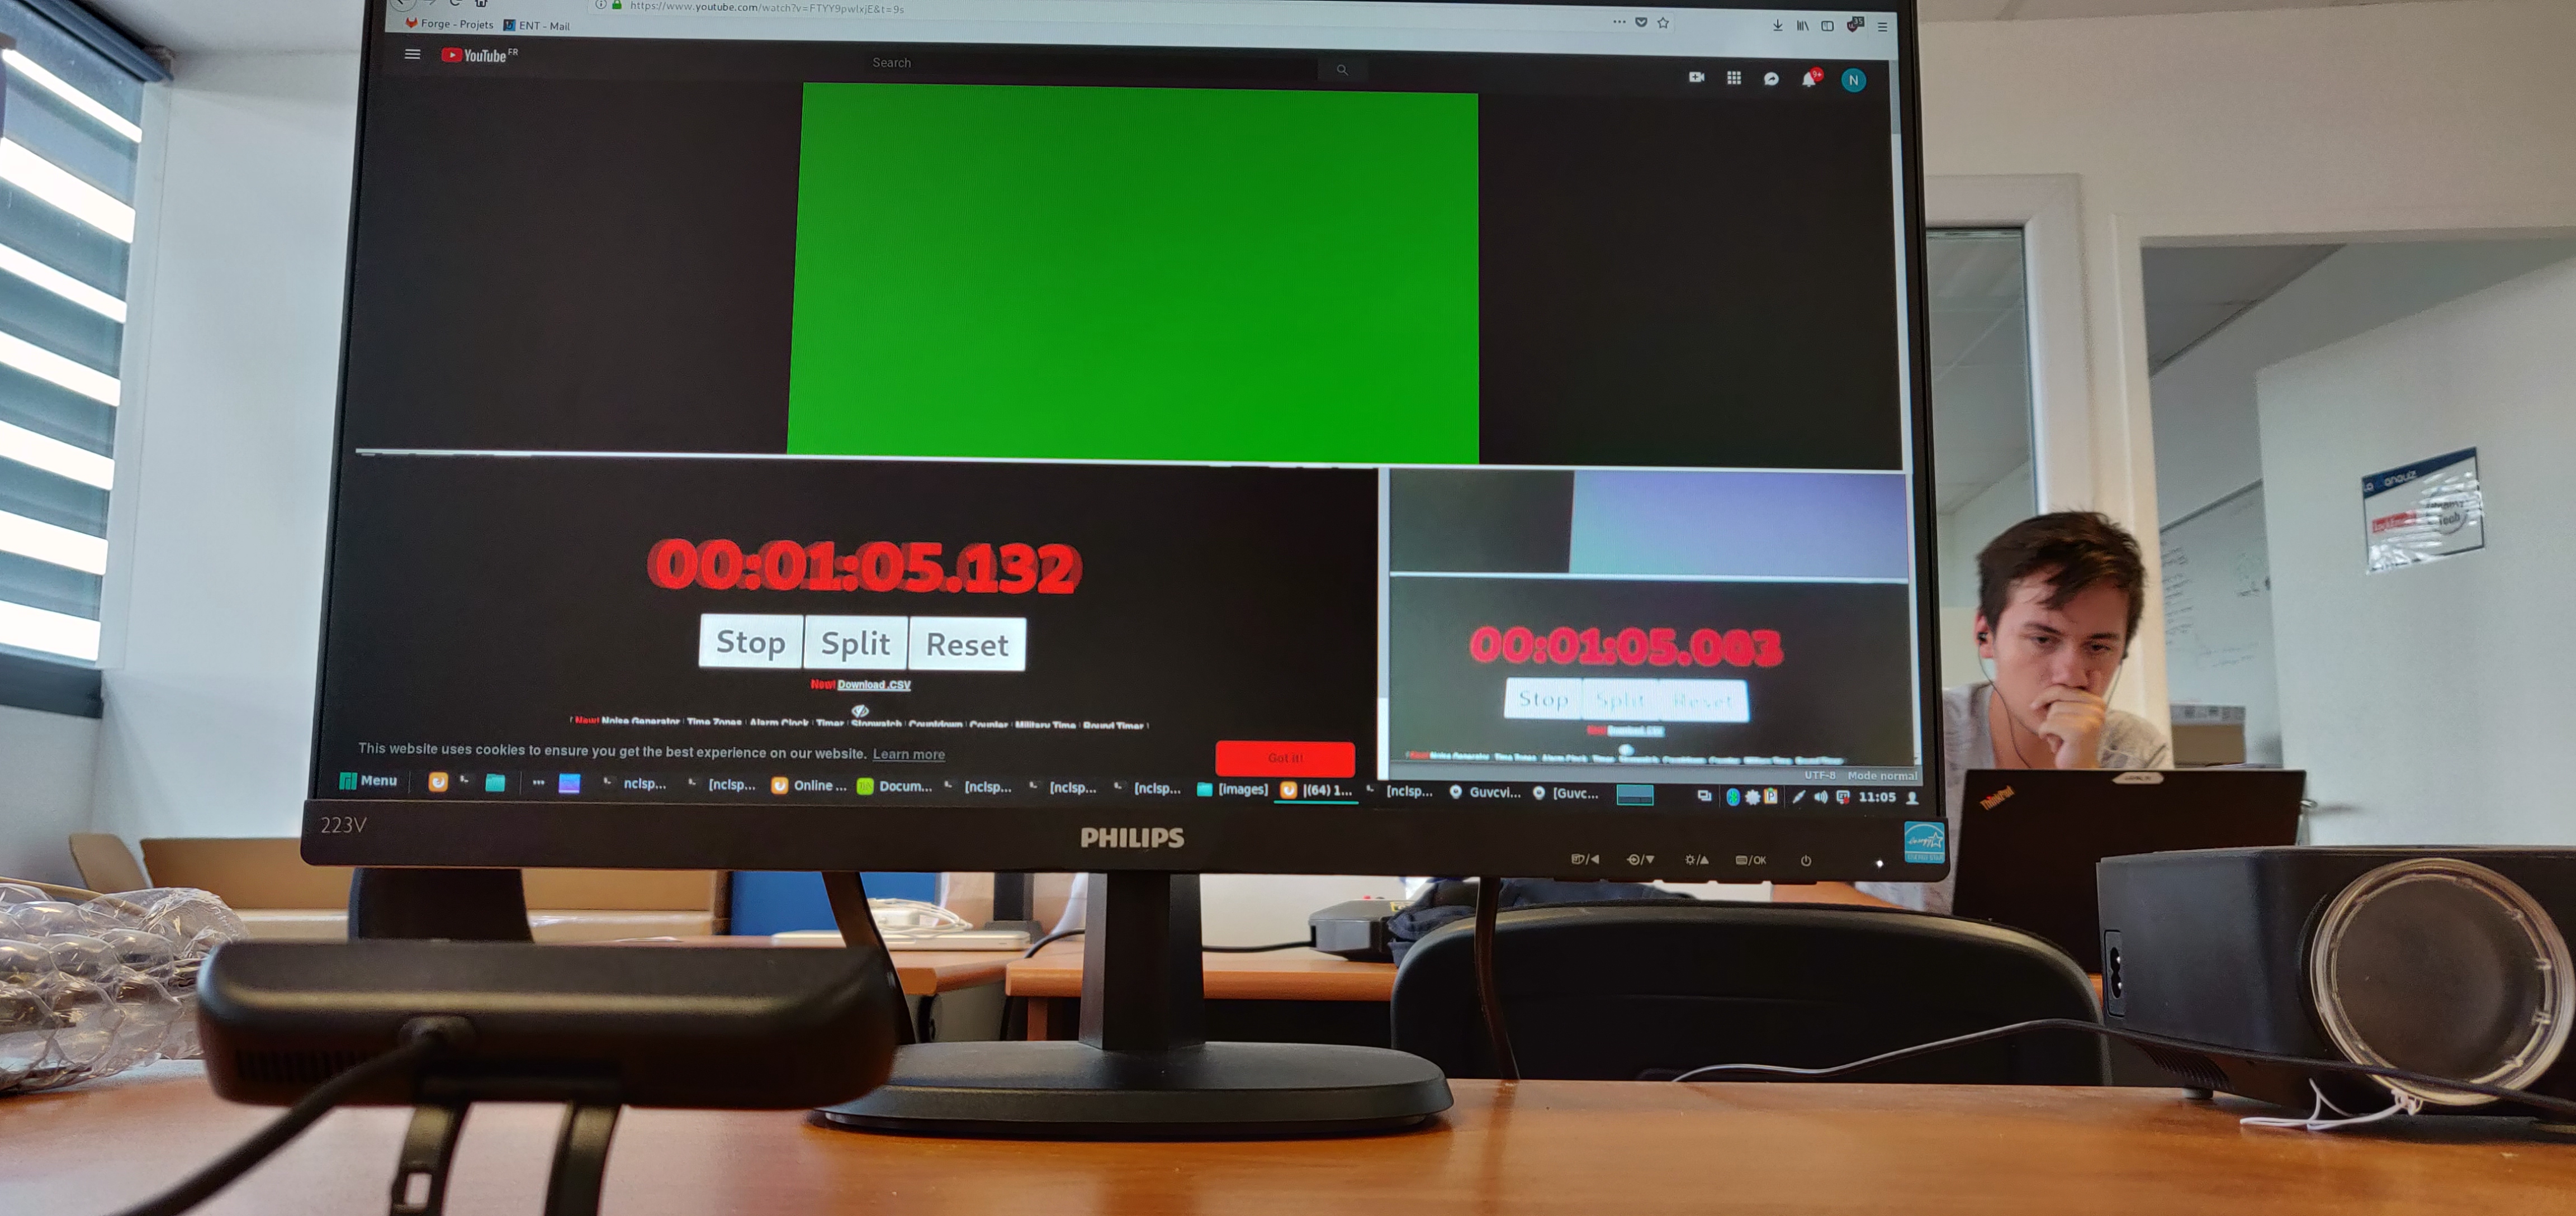
\includegraphics[width=\linewidth]{images/glasstoglass}
\caption{Exemple de mesure "glass to glass" de la latence d'une caméra}
\label{fig:latency:glasstoglass}
\end{figure}

Dans un soucis de cohérence avec la partie optimisation logicielle, vous trouverez dans le tableau~\ref{fig:latency:camera}, un comparatif des différentes latences de caméra obtenues sur le kit de développement NVIDIA Jetson TX2. Les résultats obtenus avec différents ordinateurs sont, quant à eux, présenté en Annexe 2.

\begin{table}[H]
\centering
\caption{Latence (en ms) de plusieurs caméras mesurée en Glass to glass - NVIDIA Jetson TX2}
\label{fig:latency:camera}
\resizebox{0.65\textwidth}{!}{%
\begin{tabular}{|c|c|c|c|c|c|c|}
\hline
\textbf{} & \textbf{Onboard (TX2)} & \textbf{Logitech} & \textbf{SR300} & \textbf{PSEye} & \textbf{Aukay} & \textbf{ELP} \\ \hline
\textbf{640x480} & 75 & 120 & \cellcolor{green!40} 70 & 120 & 85 & 80 \\ \hline
\textbf{1280x1020} & \cellcolor{green!40}80 & 80 & 85 & / & 85 & 85 \\ \hline
\textbf{1920x1080} & \cellcolor{green!40}80 & 130 & 300 & / & 170 & 95 \\ \hline 
\end{tabular}%
}
\end{table}

On s'aperçoit très rapidement que les tests de latence sont plutôt décevants. En effet, les latences sont toutes plus ou moins similaires même s'il y a quelques variations notamment en résolution "full HD" 1920x1080, ce qui ne permet pas d'émettre beaucoup d'hypothèse d'amélioration. On observe que même la caméra embarquée (Onboard) disposant de son propre circuit intégré sur la carte mère du TX2 n'apporte aucun gain significatif par rapport aux autres caméras.
N'étant pas satisfait des résultats, nous avons décidé de mesurer la latence d'une caméra professionnelle \texttt{Point Gray} et la latence observée a été de seulement 8-10 millisecondes avec une résolution de 1280x1020. 

Aucune réel conclusion n'a pu être tirée de ces résultats mais il s'avère que la plupart des constructeur de caméras non professionnelles n'étant pas dédié à la vision par ordinateur ne concentrent par leurs efforts sur la réduction de la latence de ces dernières mais plutôt sur l'amélioration de la qualité de l'image, la fidélité des couleurs etc.

\newpage
\section{Nectar - Architecture micro services}
\label{sec:nectararchi}

Pour achever le développement du prototype haute performance, nous avons choisi de réétudier l'architecture logicielle de PapARt. 
Actuellement, PapARt est un gros kit de développement proposant une multitude de services regroupés en son sein comme par exemple l'acquisition du flux vidéo d'une caméra, le traitement des images, la détection de marqueurs, la visualisation, l'estimation de pose, etc.. Avec la centralisation des services, une panne peut être dramatique et rendre tout le système inutilisable. L'idée était donc de développer une nouvelle architecture pour pallier à ce défaut et permettre au système de gagner en réactivité, stabilité, performance, modularité et temps de maintenance. Une architecture en micro-services s'est imposée comme solution de choix car elle répond à tous les besoins énoncés.

Une architecture en microservices consiste à décomposer un logiciel en une multitude de services indépendants, effectuant chacun une tâche bien précise. Ces services peuvent ensuite communiquer les uns avec les autres par le biais d'une API.

\paragraph{Performance} Contrairement à une bibliothèque classique, avec une telle architecture il est possible d'allouer des ressources à la demande aux services en ayant besoin. Cela permet, par exemple, d'attribuer des ressources aux services les nécessitant lorsqu'un faible nombre d'entre eux est entrain de fonctionner. A la différence d'une bibliothèque classique où les ressources supplémentaires allouées l'auraient été pour tous les services. Ce gain de performance n'est pas négligeable car il permet d'améliorer considérablement la gestion des ressources, qui peut devenir critique en cas de saturation notamment.

\paragraph{Réactivité} Dans le cas d'une panne d'un service critique, tel que le service récupérant le flux vidéo de la caméra, avec une architecture centralisée la gestion de cette panne est très complexe et nécessite souvent de redémarrer tout le système, ce qui prend un certain temps. En revanche, une architecture en microservices couplée à un gestionnaire de processus se chargera uniquement de relancer le service en panne et, s'il le faut, les services associés, de manière quasiment transparente pour l'utilisateur.

\paragraph{Modularité} L'architecture en microservices offre une très grande modularité ; chaque service peut être écrit dans n'importe quel langage et peut être intégré au système sans coût tant qu'il respecte l'API de communication inter processus s'il n'est pas totalement indépendant. Il est ainsi très facile pour n'importe qui de rajouter des modules venant soit compléter un service existant soit tout simplement rajouter une fonctionnalité au système. Par exemple, un service d'estimation de pose peut être complété par un service de filtrage de façon totalement transparente à l'utilisateur final. L'utilisation ou non du filtrage peut être contrôlée de façon automatique par un autre module gérant par exemple la qualité générale des traitements voulue par l'utilisateur.

\paragraph{Maintenabilité} Lorsqu'un service est défectueux, le problème peut être très rapidement identifié car les services sont très faiblement couplés et ainsi il n'est souvent pas nécessaire de devoir parcourir une grande quantité de code pour pouvoir identifier un bug. De plus, grâce à la modularité de l'architecture, un service en maintenance n'affecte pas la stabilité générale du système.

\begin{figure}[H]
\centering
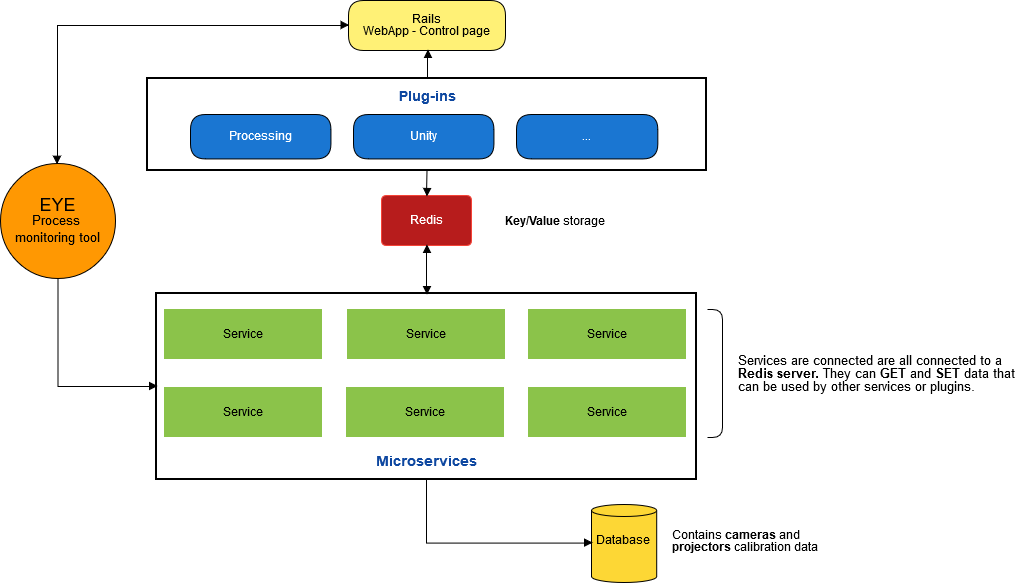
\includegraphics[width=\linewidth]{images/archi3}
\caption{Schéma de l'architecture en microservices développée}
\label{fig:microarchi}
\end{figure} 

Pour mettre en place cette nouvelle architecture (Figure~\ref{fig:microarchi}), nous nous sommes basés sur trois technologies principales :
\begin{itemize}
\item \textbf{Redis}\cite{redis} ou \emph{REmote DIctionnary Server} est un système de stockage clef-valeur qui, contrairement aux bases de données plus conventionnelles, stocke les données directement dans la mémoire vive (\emph{Random Access Memory (RAM)}) de l'ordinateur ou dans la mémoire virtuelle\footnotetext{\href{https://fr.wikipedia.org/wiki/Mémoire_virtuelle}{Wikipédia - Mémoire virtuelle}} et non pas directement sur le disque. Cette spécificité permet à Redis d'atteindre des performances inégalées par des bases de données classiques du fait du stockage en mémoire vive (bien plus rapide) et il s'impose donc comme un choix de qualité pour nos besoins.
\item \textbf{Eye}\cite{eye} est un outil de gestion de processus qui permet de s'assurer du cycle de vie des processus qu'il gère. Eye offre la possibilité de lancer/redémarrer/couper automatiquement des processus en fonction de leur état, de leur dépendance et de leur consommation en ressource (mémoire, CPU). Il est ainsi possible de définir, pour chaque service, de quoi il dépend et quelles sont les ressources maximales qui lui sont autorisées, ce qui permet d'éviter la mise en péril de tout le système lorsqu'un processus commence à consommer 99\% de la mémoire disponible par exemple.
\item \textbf{Ruby on Rails}\cite{rubyrails} est un \emph{framework} destiné à la création d'applications web modernes rapidement et simplement. L'idée est d'utiliser Rails pour générer une page web de contrôle du système permettant de lancer/couper des processus, effectuer des tests et tout autre action permettant d'observer l'état général du système.
\end{itemize}

Dans notre architecture, tous les microservices sont connectés à Redis. Ils peuvent chacun manipuler les données présentes et en écrire de nouvelles. C'est uniquement par ce biais que se fait la communication inter services. Ainsi, par exemple, un service accédant à la caméra ne transfère pas directement ses données à un service analysant l'image, mais envoie l'image courante de la caméra dans Redis qui est ensuite récupérée par cet autre service. En outre, Redis possède une pipeline événementiel. Ce pipeline permet aux clients Redis (services) écoutant ou publiant sur une clé de notifier ou d'être notifié d'autres / par d'autres services. De ce fait, dès que des nouvelles données seront publiées sur une clé écoutée par des clients, ceux-ci recevront instantanément lesdites données. C'est ce pipeline que nous avons choisi d'utiliser pour éviter l'attente active des services et ainsi améliorer les performances générales du système.
Le phénomène d'attente active ce présente lorsqu'un processus vérifie constamment si une condition est vraie. Dans notre cas la condition pourrait être "est ce que des nouvelles données sont disponibles ?". Cette attente n'est pas bénéfique pour le système car les ressources sont précieuses et limitées et ainsi un processus ne peut se permettre de monopoliser ces derniers sous prétexte de vérifier si des nouvelles données sont arrivées d'où l'utilisation du pipeline événementiel.

Couplé à Redis, c'est Eye qui s'assure à tout moment que tous les services demandés par l'utilisateur sont en train d'être exécutés. Pour cela, il vérifie que le service est en marche mais aussi que toutes les dépendances sont satisfaites. Eye peut recevoir des commandes de l'application web qui est elle-même manipulée, soit par l'utilisateur soit par un module de développement. Les modules de développement sont des API permettant aux utilisateurs développeurs de créer leurs propres applications de réalité augmentée spatiale utilisant le système de RealityTech.

\section{Bilan}
Après avoir réalisé puis testé indépendamment chacune des parties composant le prototype haute performance, la dernière étape consistait à tester ce dernier, de bout en bout, dans un cas d'utilisation réelle. Le but de cet ultime test étant d'évaluer si le prototype remplit, ou non, les objectifs que nous nous sommes fixés à savoir : performance, réactivité, modularité et maintenabilité. 
Pour effectuer ce test, il fallait développer une application utilisant ce prototype. Pour ce faire, nous avions besoin du module Unity le mettant à profit. Le développement du module Unity ainsi que de l'application est détaillé Chapitre~\ref{chap:unity}.
A ce jour, le module et l'application n'étant toujours pas terminés, le test n'a pas encore été réalisé.


\newpage

%récupérer les citation avec "/footnotemark"
\nocite{*}

%choix du style de la biblio
\bibliographystyle{plain}
%inclusion de la biblio
\bibliography{bibliographie}
%voir wiki pour plus d'information sur la syntaxe des entrées d'une bibliographie

\end{document}